\chapter{Streszczenie}
\label{cha:elementyPracyproj}

\section{Streszczenie}
Dokumentacja aplikacji desktopowej wspomagającej zarządzanie budynkiem mieszkalnym. 
Aplikacja umożliwia administratorowi zarządzanie informacjami o m.in. lokatorach oraz zgłoszeniach. 
Projekt został wykonany w języku Java z wykorzystaniem biblioteki Swing (interfejs graficzny) oraz JDBC z Connector J do komunikacji z bazą danych MySQL. 
Aplikacja oferuje zarządzanie mieszkaniami, przypisanie właściciela do mieszkań, odbieranie zgłoszeń od mieszkańców,
dodawanie/usuwanie mieszkańców/mieszkań, modyfikowanie parametrów mieszkań.

\section{Summary}
Documentation of a desktop application supporting the management of a residential building. 
The application allows the administrator to manage informations like, tenants and notifications. 
The project was made in Java using the Swing library (graphical interface) and JDBC with Connector J for communication with the MySQL database. 
The application offers apartment management, assigning owners to apartments, receiving notifications from residents, 
adding/removing residents/apartments, modifying apartment parameters.

\newpage
\chapter{Opis założeń projektu}
\section{Cel projektu}
Celem projektu było stworzenie aplikacji desktopowej która pomogła by w zarządzaniu budynkiem mieszkalnym. Projekt ten miał być 
stworzony przy użyciu języka obiektowego Java (wersja Oracle OpenJDK 24.0.1) wraz z prostą oprawą graficzną poprzez bibliotekę Swing.
Projekt miał się łączyć z bazą danych przy użyciu JDBC wraz z modułem Connector J (wersja 9.3.0). Aplikacja ta miała pozwalać 
administratorowi budynku na dodawanie lub usuwanie użytkowników, mieszkań oraz zarządzanie mieszkaniami.

%----------------Funkcjonalne
\section{Wymagania funkcjonalne}
\begin{enumerate}
    \item \textbf{Logowanie, rejestracja użytkowników} - użytkownicy posiadają swój numer PIN jako hasło oraz unikalną nazwę użytkownika żeby logować sie do systemu
    \item \textbf{Zarządzanie parametrami mieszkania} - użytkownik może zmieniać temperaturę wody i powietrza, włączać i wyłączać zasilanie, światło w mieszkaniu
    \item \textbf{Otwieranie/zamykanie budynku}
    \item \textbf{Zarządzanie użytkownikami}
        \begin{itemize}
            \item dodawanie użytkownika
            \item usuwanie użytkownika
        \end{itemize}
    \item \textbf{Zarządzanie mieszkaniami}
        \begin{itemize}
            \item dodawanie mieszkań
            \item usuwanie mieszkań
            \item przydzielanie właściciela mieszkania
            \item usuwanie właściciela mieszkania
        \end{itemize}
    \item \textbf{Przechowywanie zgłoszeń mieszkańców}
        \begin{itemize}
            \item tworzenie zgłoszeń
            \item usuwanie zgłoszeń
        \end{itemize}
\end{enumerate}

%----------------Niefunkcjonalne
\section{Wymagania niefunkcjonalne}
\begin{enumerate}
    \item \textbf{Niezależność od systemu operacyjnego} - dzięki Java \cite{Java} JVM (wersja nie niższa niż OpenJDK 24.0.1) program działa na systemach takich jak Windows, Linux, MacOS. 
    \item \textbf{Intuicyjność} - program łatwy w użytku dzięki oprawie graficznej \cite{Java2}
    \item \textbf{Responsywność} - program szybko reaguje na operacje wykonywane przez użytkownika
\end{enumerate}

%----------------Sprzętowe
\section{Wymagania sprzętowe}
\begin{enumerate}
    \item \textbf{Java} - OpenJDK 24.0.1
    \item \textbf{IntelliJ} - IDE do uruchomienia projektu
    \item \textbf{Connector J (wersja 9.3.0)} - połączenie IntelliJ z bazą danych
    \item \textbf{Xampp} - lokalna konfiguracja bazy danych
\end{enumerate}
%--------------OPIS STRUKTURY
\chapter{Opis struktury projektu}
\section{Zdalne repozytorium projektu}
Projekt jest przechowywany na zdalnym repozytorium na stronie github.com pod adresem 
\newline \url{https://github.com/K4-pi/Java/tree/main/Projekt} w folderze \textit{BuildingManagment}.

\section{Baza danych}
\subsection{Konfiguracja bazy danych (Xampp)}
Do poprwanego działania aplikacji konieczne jest połączenie z bazą danych.
Połączenie z bazą należy wykonać przy użyciu narzędzia Xampp dostępnego na stronie 
\url{https://www.apachefriends.org/pl/index.html} patrz rysunek 3.1 
(w tym przykładzie użyto wersji 3.3.0).

\begin{figure}[H]
    \centering
    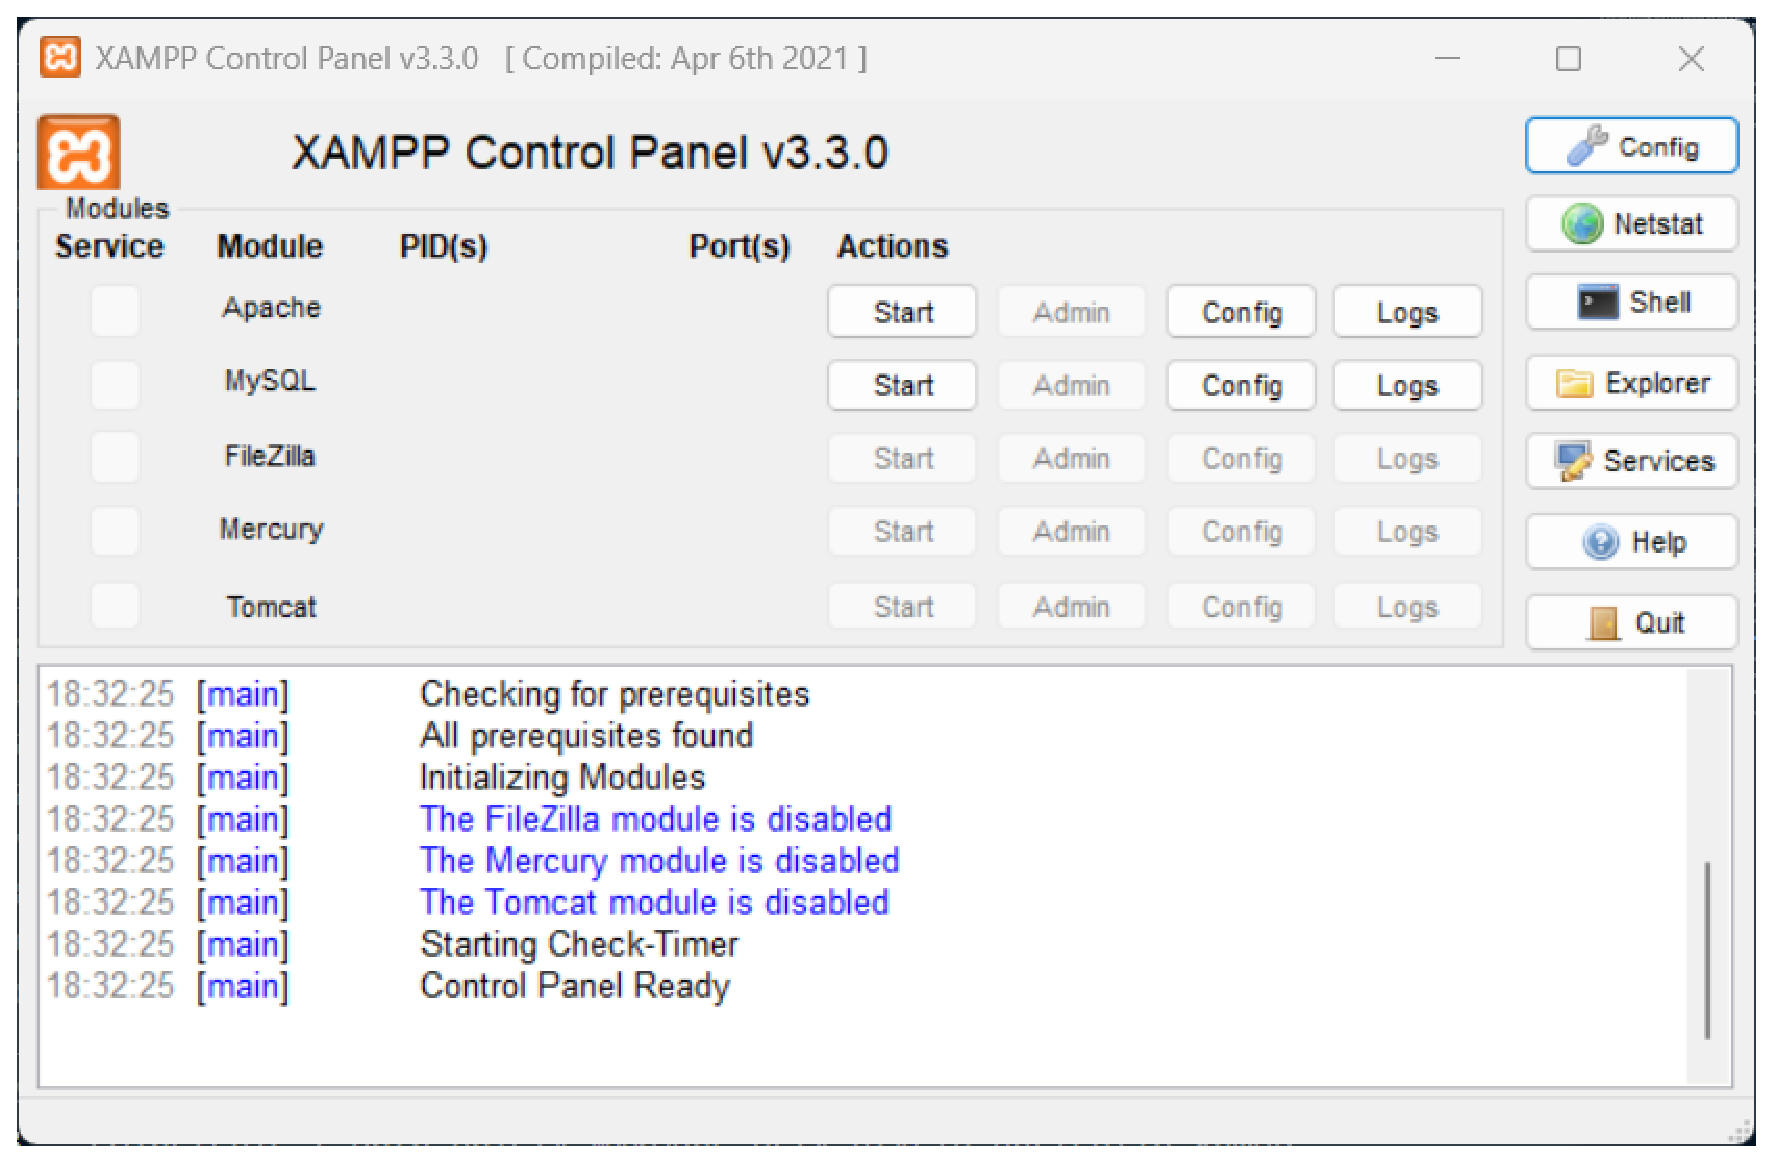
\includegraphics[width=\linewidth]{figures/xampp.eps}\\
    \caption{Aplikacja Xampp.\label{fig1}}
\end{figure}

\newpage
\noindent Następnie poprzez aplikacje Xampp należy włączyć moduł Apatche oraz MySQL
\textcolor{red}{UWAGA!} Należy się upewnić, że moduł MySQL działa na porcie 3306.
Poprzez panel phpMyAdmin (Rys 3.2) włączany przez przycisk \textit{Admin} znajdujący się w aplikacji
Xampp przy module MySQL lub przez adres URL  \url{http://localhost/phpmyadmin/index.php}.
Następnie należy stworzyć baze danych o nazwie \textit{building} i zaimportować
do niej plik o nazwie \textit{building.sql} dołączony do plików projektu.

\begin{figure}[H]
    \centering
    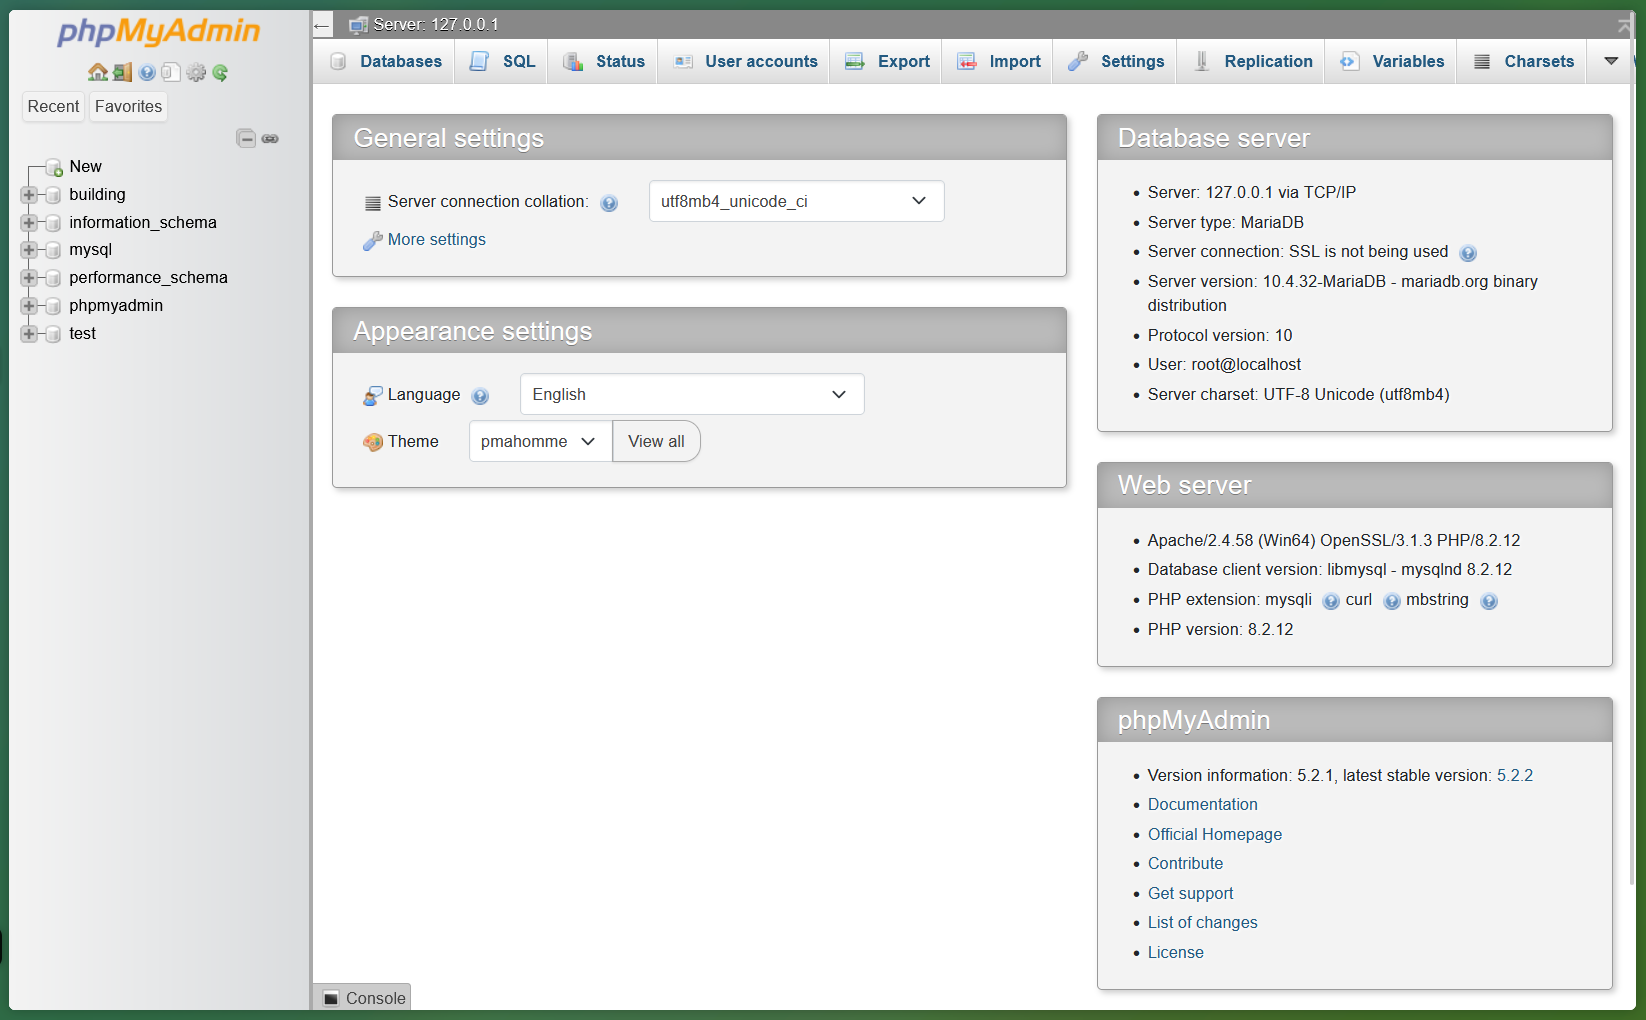
\includegraphics[width=\linewidth]{figures/phpadmin.eps}\\
    \caption{phpMyAdmin.\label{fig2}}
\end{figure}

%\listingname~\ref{databaseconnection} Połączenie z bazą danych.
\noindent Nawiązując do kodu Java dzięki któremu aplikacja łączy się z bazą danych (Listing 3.1)
musimy zrobić w stworzonej przez nas bazie danych \textit{building} użytkownika o nazwie \textit{app} z hasłem \textit{1234} z uprawnieniami administratora.
\lstinputlisting[caption= Połączenie z bazą danych, label=databaseconnection, style = csStyle]{src/DatabaseConnection.java}

\subsection{IntelliJ}
Jeżeli chcemy włączyć aplikacje poprzez program IntelliJ potrzebujemy Java OpenJDK wersję conajmniej 24.0.1 oraz Connector J (w projekcie użyto wersji 9.3.0)
dostępny na stronie \url{https://dev.mysql.com/downloads/connector/j/}.
Po pobraniu musimy zaimportować moduł do projektu poprzez zakładkę \textit{File > Project structure > Modules} i dodać moduł (patrz rys. 3.3).

\begin{figure}[H]
    \centering
    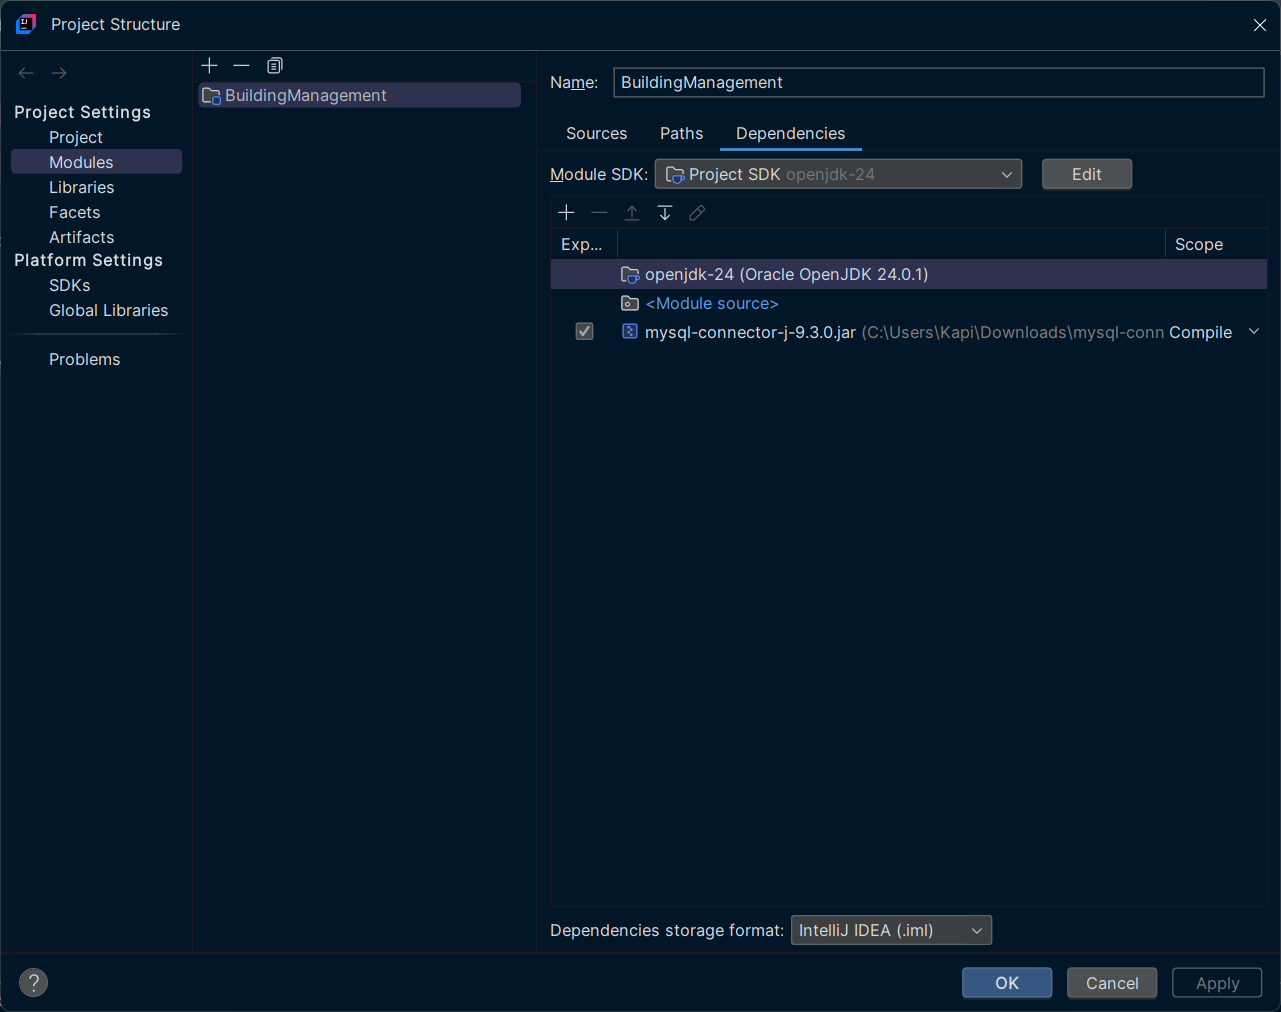
\includegraphics[width=\linewidth]{figures/project-struct.eps}\\
    \caption{IntelliJ - Connector J\label{fig3}}
\end{figure}

\subsection{Struktura tabel bazy danych}

\begin{figure}[H]
    \centering
    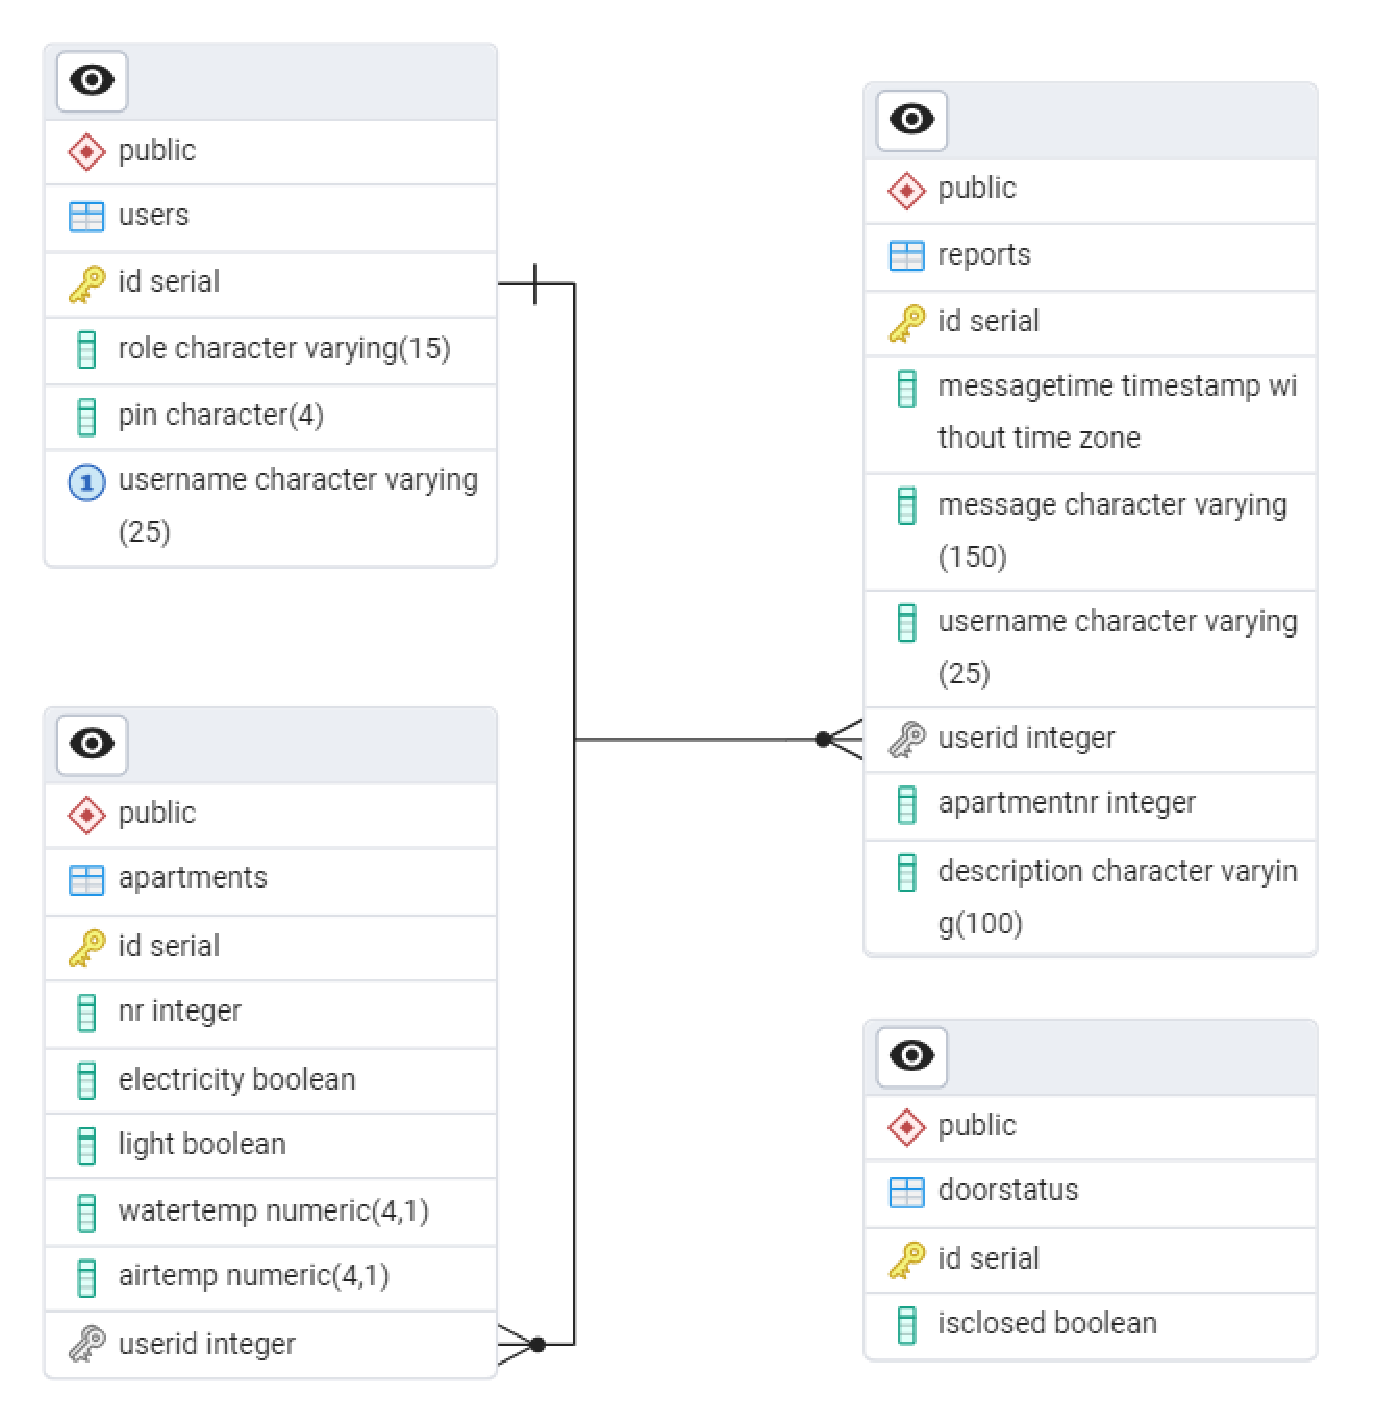
\includegraphics[width=\linewidth]{figures/database.eps}\\
    \caption{Baza danych.\label{fig4}}
\end{figure}

\newpage \section{Struktura klas programu}
\noindent Klasy dziedziczące po klasie \textit{Window} (Rys. 3.5):
\begin{itemize}
    \item AdminPanel
    \item UserPanel
    \item ReportPanel
\end{itemize}

\begin{figure}[H]
    \centering
    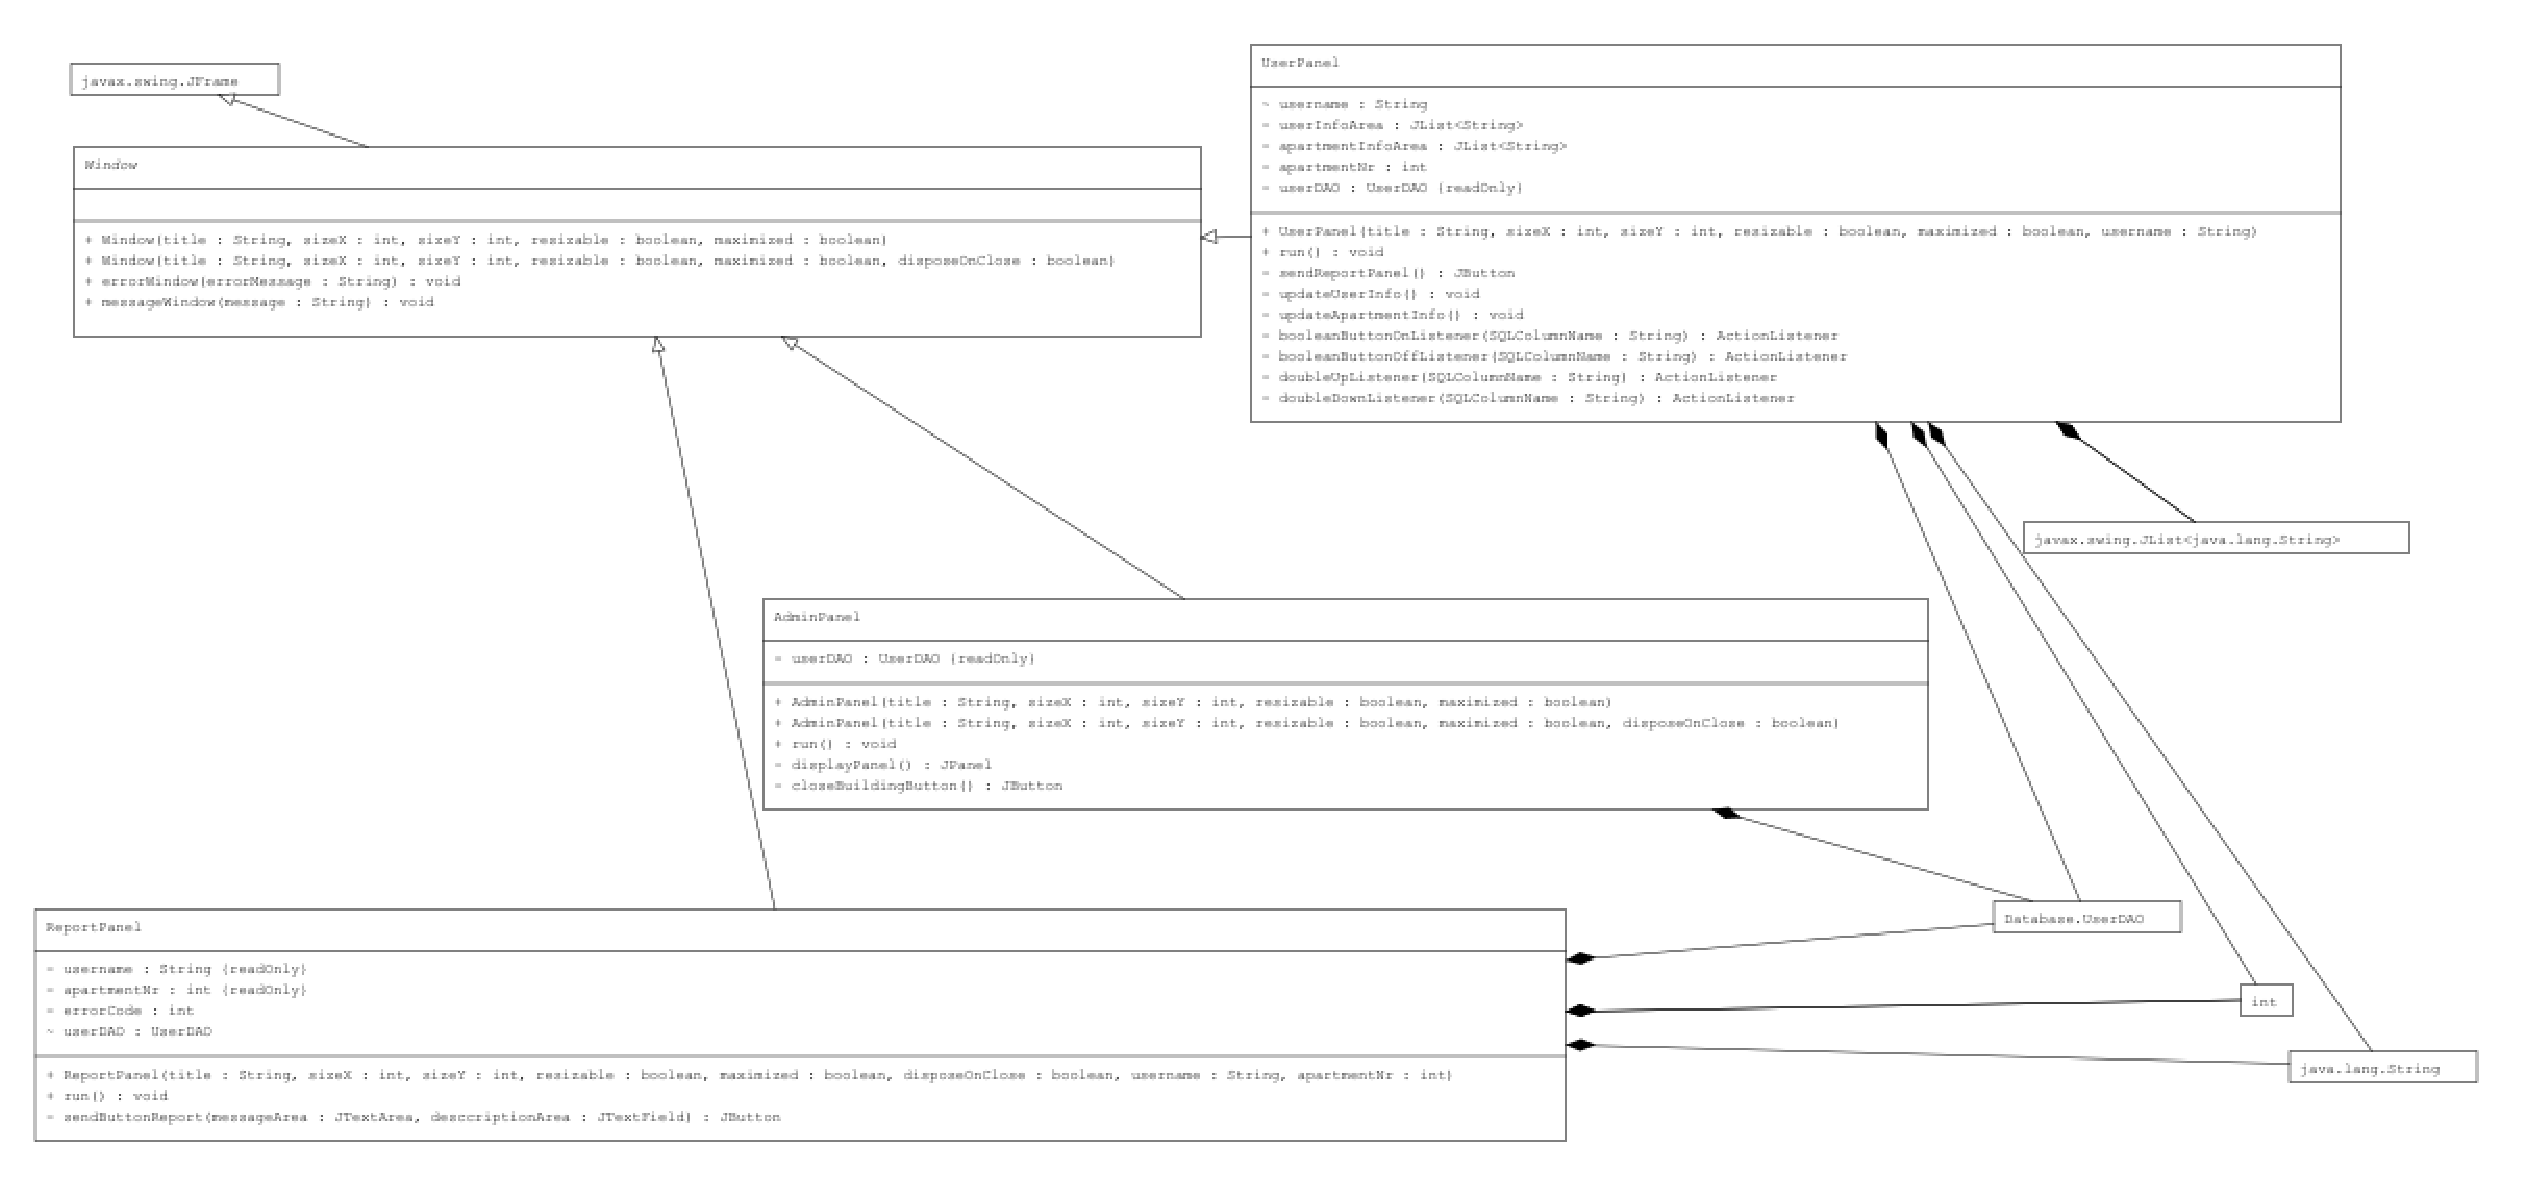
\includegraphics[width=\textwidth,height=1\textheight,keepaspectratio]{figures/UML/main-panels.eps}
    \caption{Klasa Window.\label{fig23}}
\end{figure}

\noindent Klasy dziedziczące po klasie \textit{AdminPanel} (Rys. 3.6):
\begin{itemize}
    \item Add
    \item Remove
    \item ApartmentPanel
    \item ReportMessageWindow
\end{itemize}

\begin{figure}[H]
    \centering
    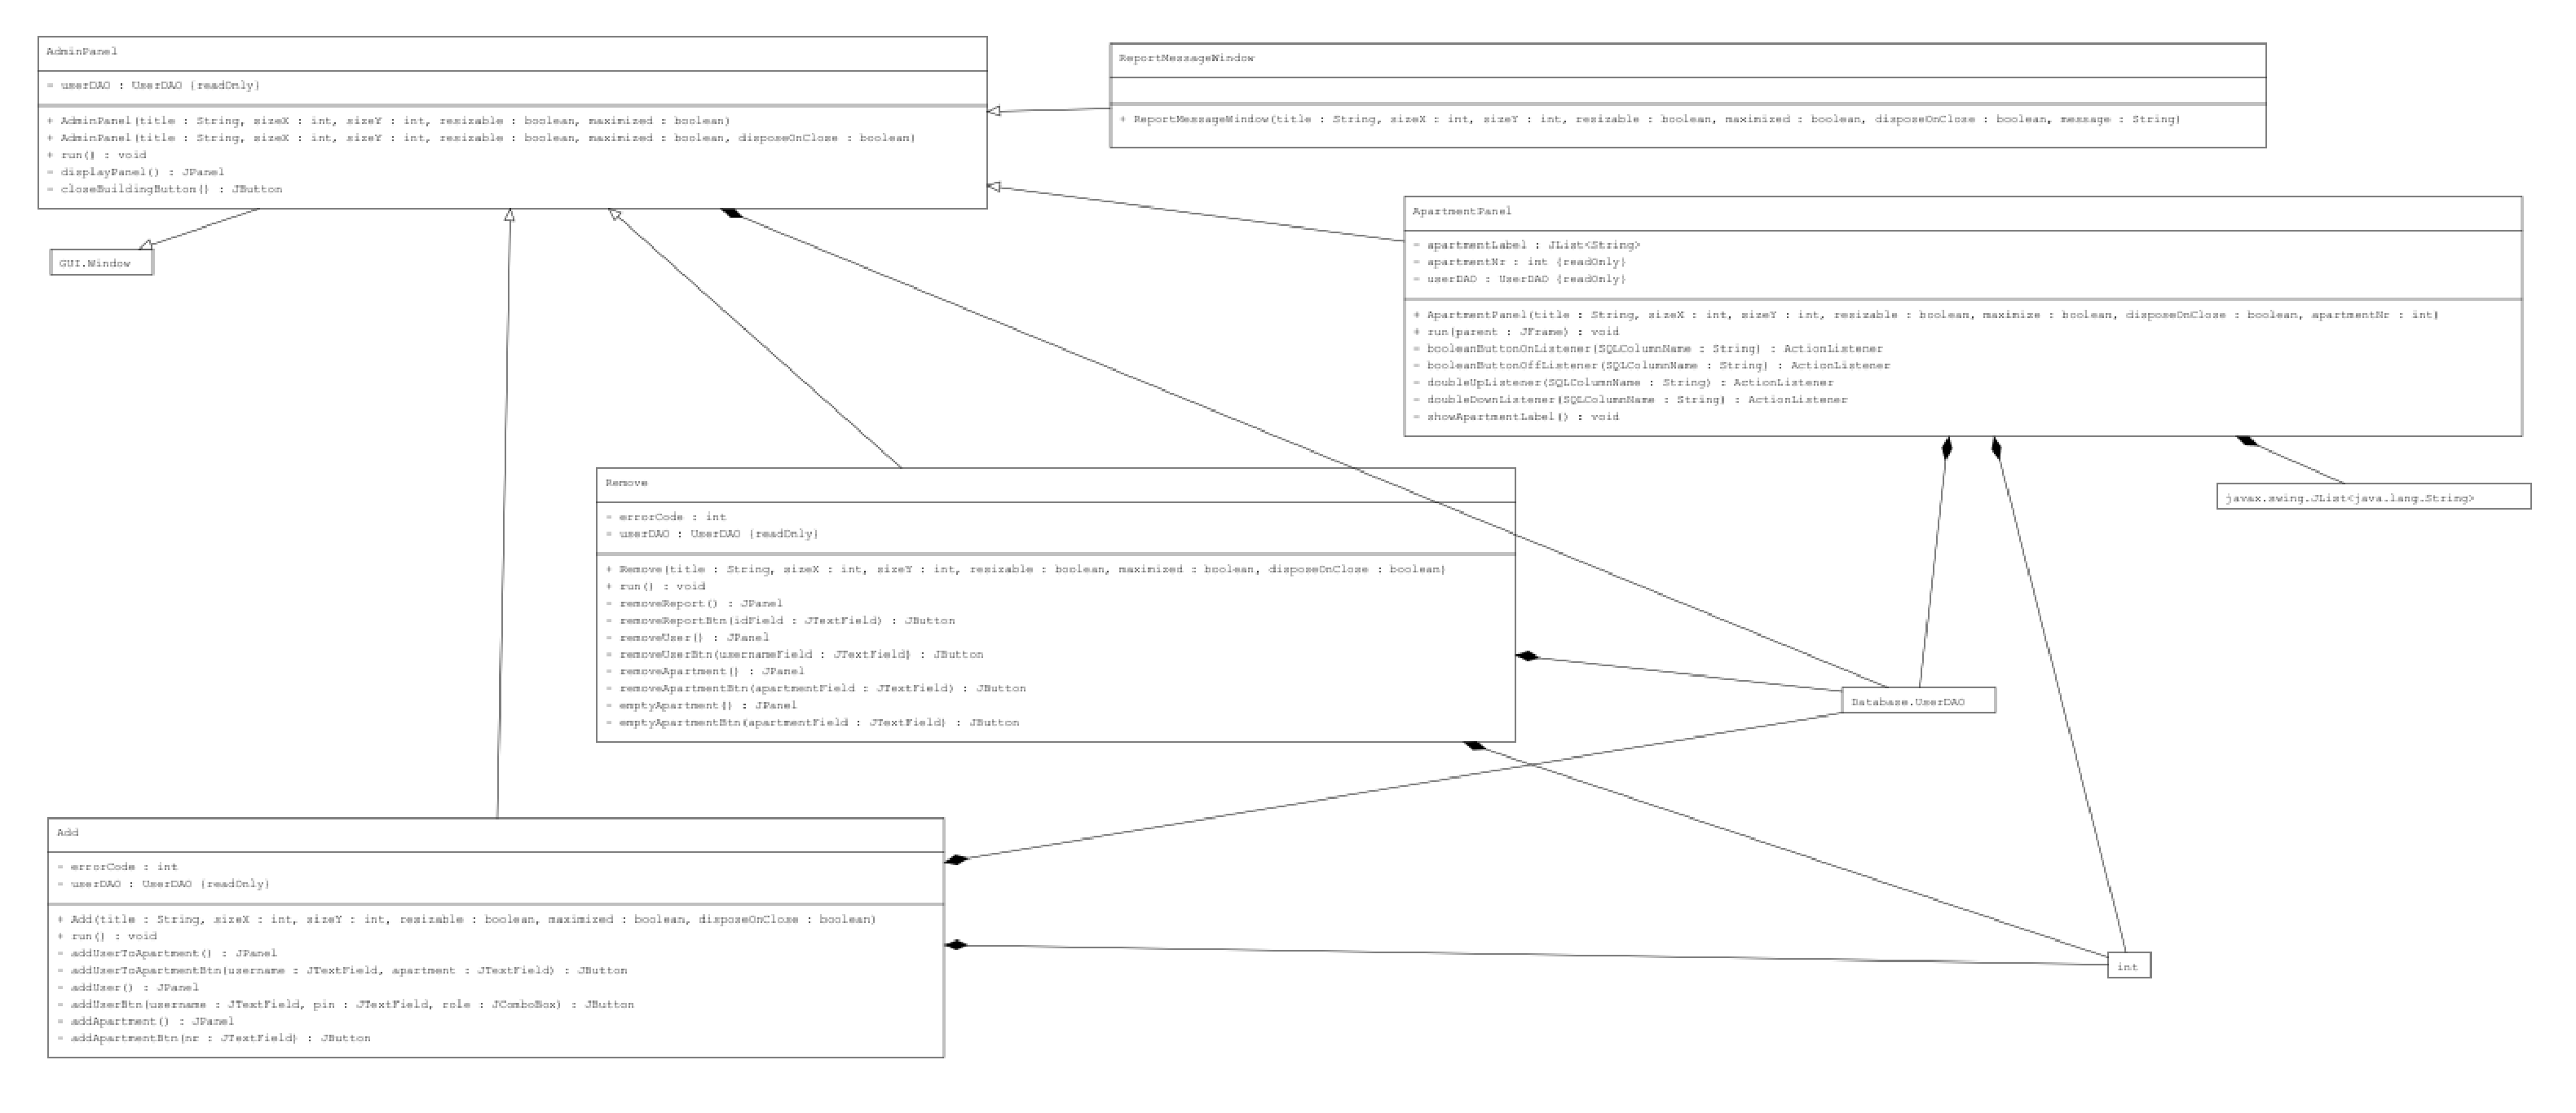
\includegraphics[width=\textwidth,height=1\textheight,keepaspectratio]{figures/UML/admin-extends.eps}
    \caption{Klasa AdminPanel.\label{fig24}}
\end{figure}

\newpage
\section{Najważniejsze klasy programu}
\subsection{Klasa Window}
Klasa abstrakcyjna która dziedziczy po klasie \textit{JFrame}, po klasie \textit{Window} (Listing 3.2) dziedziczą takie klasy jak \textit{AdminPanel} i \textit{UserPanel}.
\lstinputlisting[caption= Klasa Window, label=Window, style = csStyle]{src/Window.java}

\newpage
\subsection{Klasa Main}
Klasa \textit{Main} (Listing 3.3) w której rozpoczyna się program.
\lstinputlisting[caption= Klasa Main, label=main, style = csStyle]{src/main.java}

\subsection{Weryfikacja użytkownika}
Przy próbie logowania program wysyła zapytanie do bazy danych (Listing 3.4 i 3.5) i weryfikuje istnienie użytkownika oraz jego role na podstawie podanej
nazwy użytkownika oraz numeru PIN, trzeba pamiętać, że nazwa użytkownika nie powtarza się w bazie danych. Jeżeli dane znajdują się 
w bazie danych to na podstawie roli użytkownik zostaje dopuszczony do panelu admina bądź zwykłego użytkownika, ponadto administrator 
może w panelu zamknąć budynek a wtedy zwykły użytkownik nie ma dostępu do budynku.
\lstinputlisting[caption= Klasa Entry, label=databaseconnection, style = csStyle]{src/UserLogin/UserLogin.java}

\newpage
\lstinputlisting[caption= Klasa UserDAO - zapytanie do bazy danych, label=databaseconnection, style = csStyle]{src/UserLogin/authenticate.java}

\subsection{Dodawanie elemntów przez administratora}
W klasie \textit{Add} zdefiniowane są funkcje, które pozwalają administratorowi na dodawanie elementów do bazy danych (Listingi 3.6, 3.7, 3.8).
\lstinputlisting[caption= Dodawanie użytkownika do apartamentu, label=databaseconnection, style = csStyle]{src/Add/addUserToApartment.java}
\newpage \lstinputlisting[caption= Dodawanie użytkowników, label=databaseconnection, style = csStyle]{src/Add/addUser.java}
\lstinputlisting[caption= Dodawanie mieszkań, label=databaseconnection, style = csStyle]{src/Add/addApartment.java}

\newpage
\subsection{Usuwanie elemntów przez administratora}
W klasie \textit{Remove} zdefniowane są funkcje pozwalające administratorowi na usuwanie elementów z bazy danych (Listingi 3.9, 3.10, 3.11)
\lstinputlisting[caption= Usuwanie użytkownika z mieszkania, label=databaseconnection, style = csStyle]{src/Remove/RemoveUserFromApartment.java}
\lstinputlisting[caption= Usuwanie użytkownika, label=databaseconnection, style = csStyle]{src/Remove/RemoveUser.java}
\newpage \lstinputlisting[caption= Usuwanie mieszkania, label=databaseconnection, style = csStyle]{src/Remove/RemoveApartment.java}
\lstinputlisting[caption= Usuwanie zgłoszenia użytkownika, label=databaseconnection, style = csStyle]{src/Remove/RemoveReport.java}

%--------------------Harmonogram

\chapter{Harmonogram realizacji projektu}
\section{System kontroli wersji}
Do realizacji projektu użyto aplikacji Git jako system kontroli wersji 
a repozytorium z projektem jest zapisane zdalnie na platformie Github pod adresem
\url{https://github.com/K4-pi/Java/tree/main/Projekt}.
Diagram Gantta przedstawia etapy pracy nad projektem.

\section{Diagram Gantta}
\begin{figure}[H]
    \center
    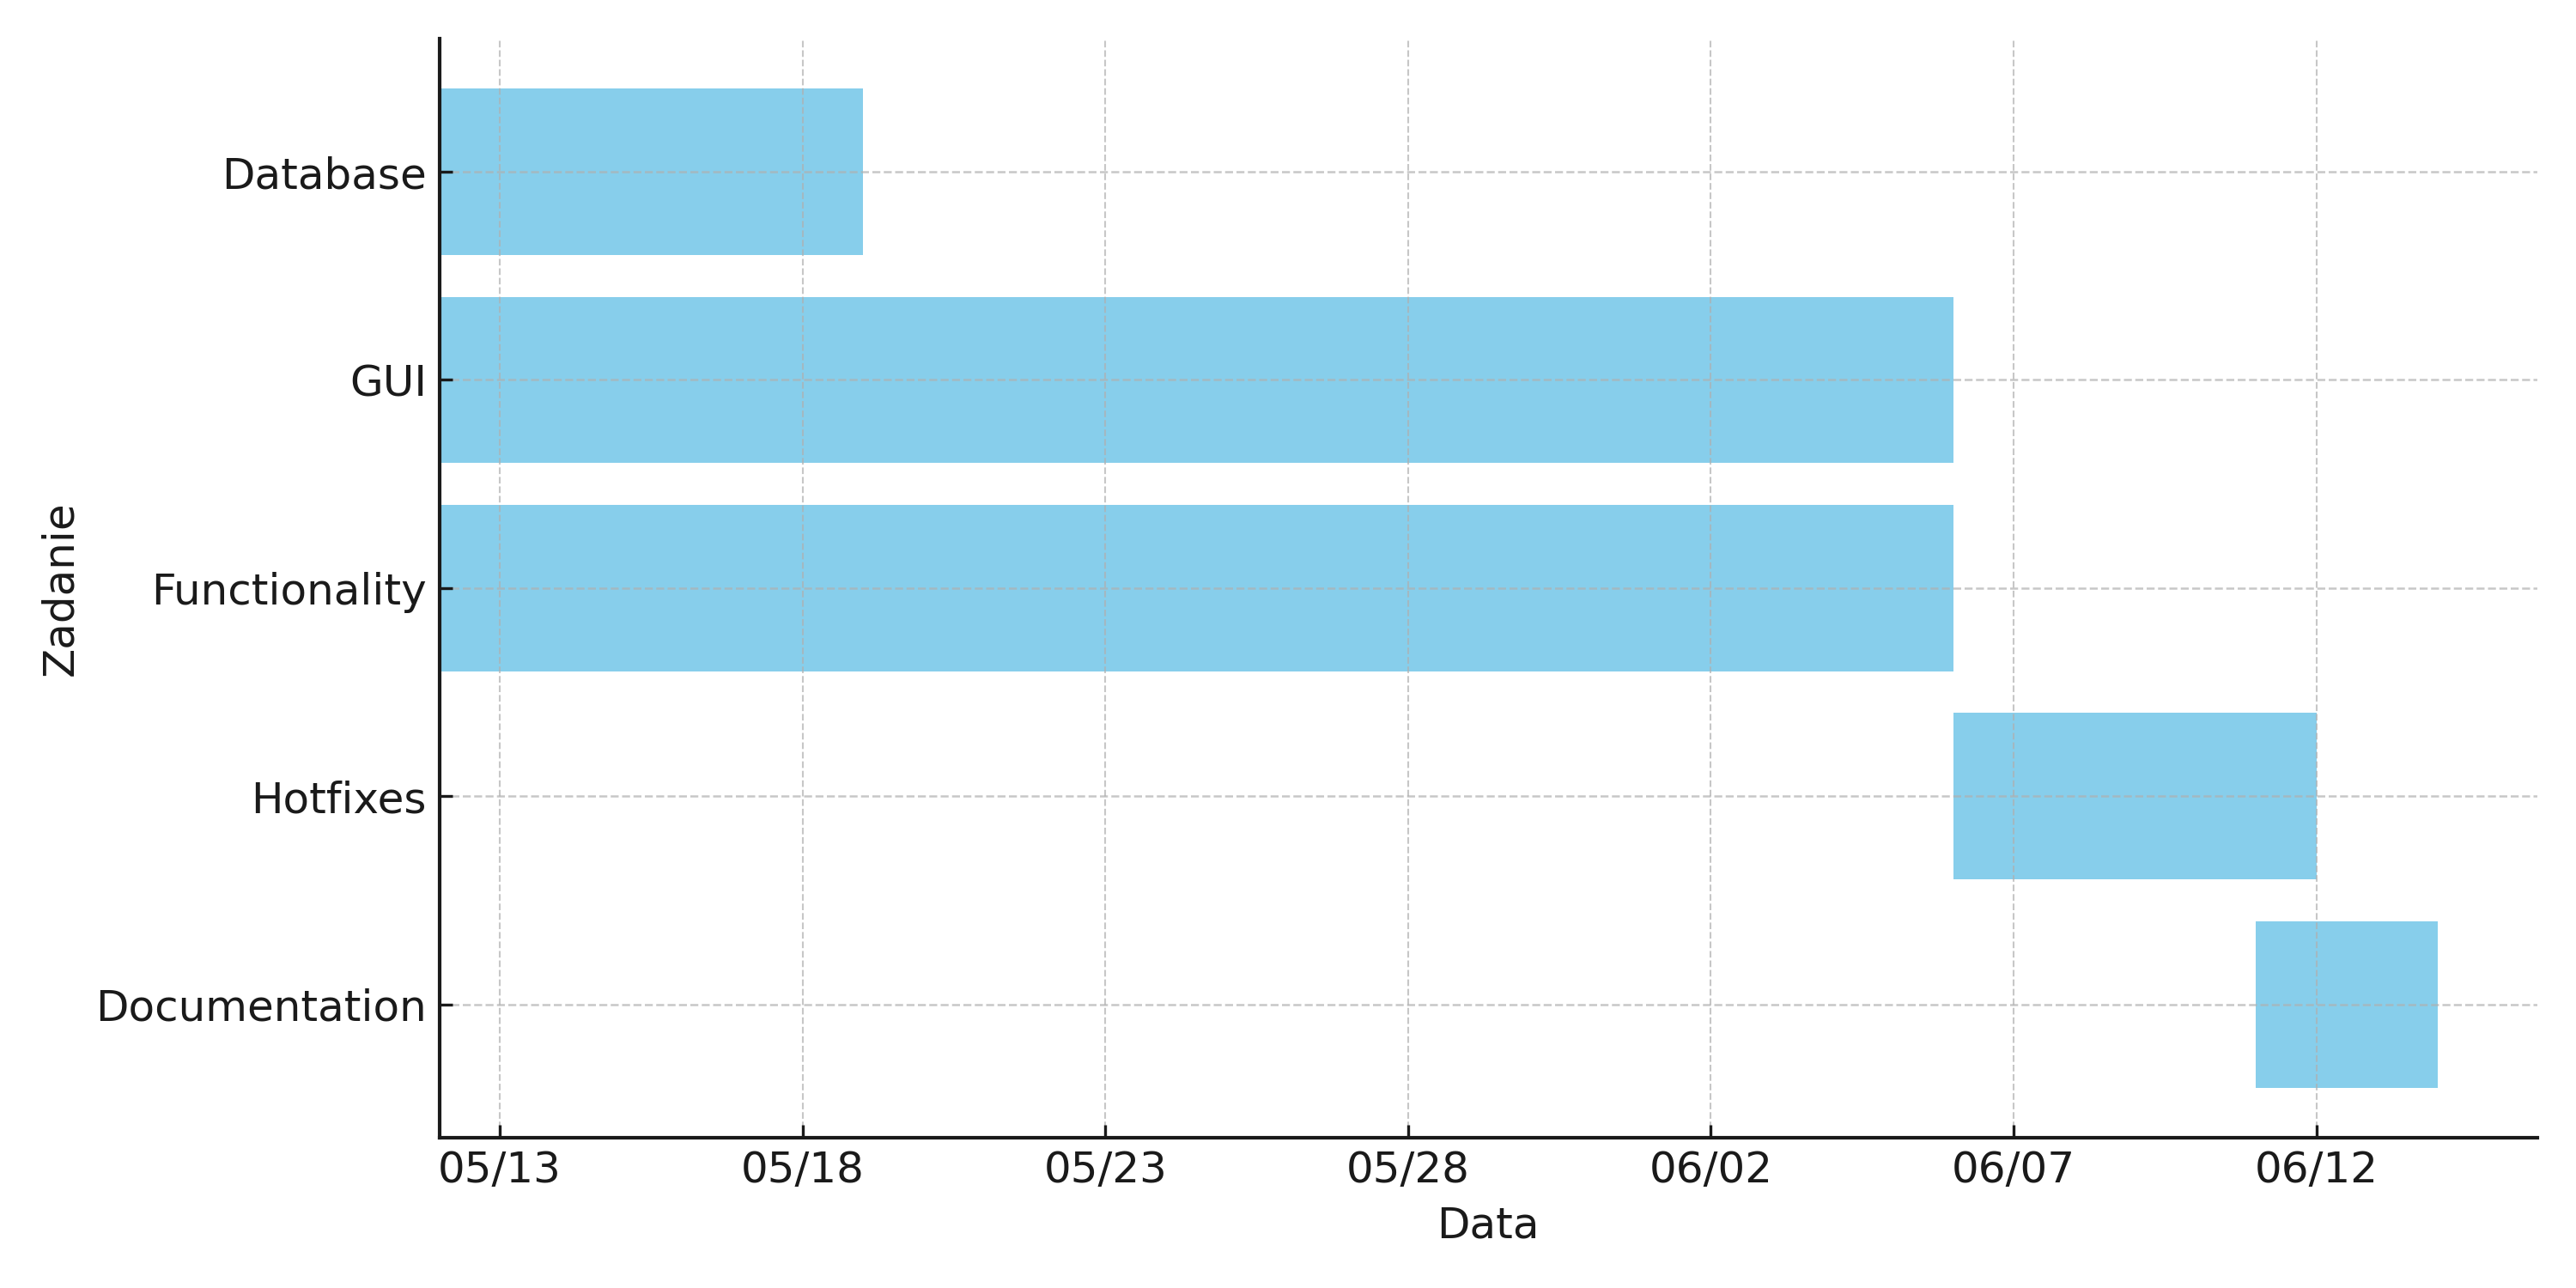
\includegraphics[width=\linewidth]{figures/Gantt-EN.eps}\\
    \caption{Diagram Gantta \cite{Gan24} (miesiąc-dzień).\label{fig5}}
\end{figure}

%-------Warstwa użytkowa
\newpage
\chapter{Warstwa użytkowa projektu}
\section{Opis}
Building Manager to aplikacja pozwalająca na łatwe zarządzanie budynkiem mieszkalnym. Oferuje takie funkcje jak dodawanie/usuwanie użytkowników, 
mieszkań, zgłoszeń.

\section{Okna informacyjne}
Są to okna wyświetlane gdy operacja nie może zostać wykonan z jakiegoś powodu jak na przykład gdy użytkownik poda nieprawidłowe dane (Rys. 5.1), 
lub po prostu informuje o wykonaniu pewnego rodzaju zadania (Rys 5.2).

\begin{figure}[H]
    \centering
    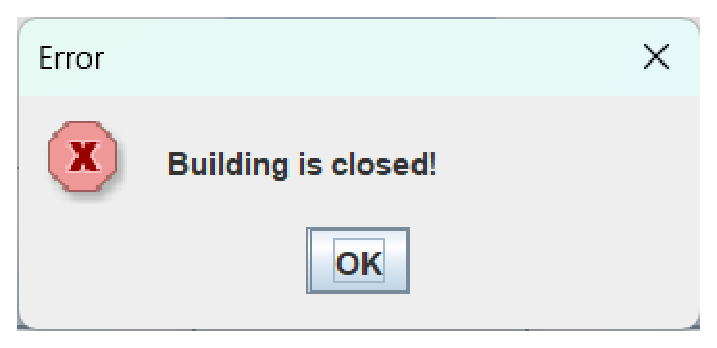
\includegraphics[width=\textwidth,height=0.2\textheight,keepaspectratio]{figures/app-images/closed-building.eps}
    \caption{Okno błędu. \label{fig6}}
\end{figure}

\begin{figure}[H]
    \centering
    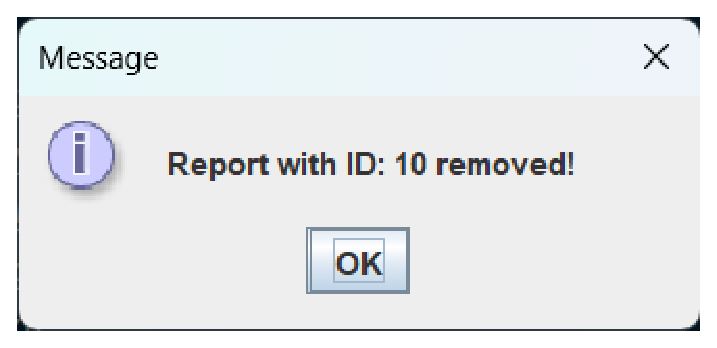
\includegraphics[width=\textwidth,height=0.2\textheight,keepaspectratio]{figures/app-images/info.eps}
    \caption{Okno informacyjne. \label{fig7}}
\end{figure}

\newpage
\section{Ekran logowania}
\subsection{Dane konta admina}
\noindent Domyślnymi danymi konta administratora są: 
\newline login: \textbf{admin}
\newline PIN: \textbf{9999}

\subsection{Panel logowania}
Jest to pierwsze okno które jest wyświetlane po uruchomieniu aplikacji (Rys. 5.3). Użytkownik może wporwadzić tu swój login oraz PIN w celu
zalogowania się do systemu. Jeżeli rola użytkownika zdefiniowana w bazie danych to \textit{admin}, użytkownik 
zostanie zalogowany do panelu admina jeśli zaś jego rola to \textit{user}, zostanie zalogowany do panelu mieszkańca.

\begin{figure}[H]
    \centering
    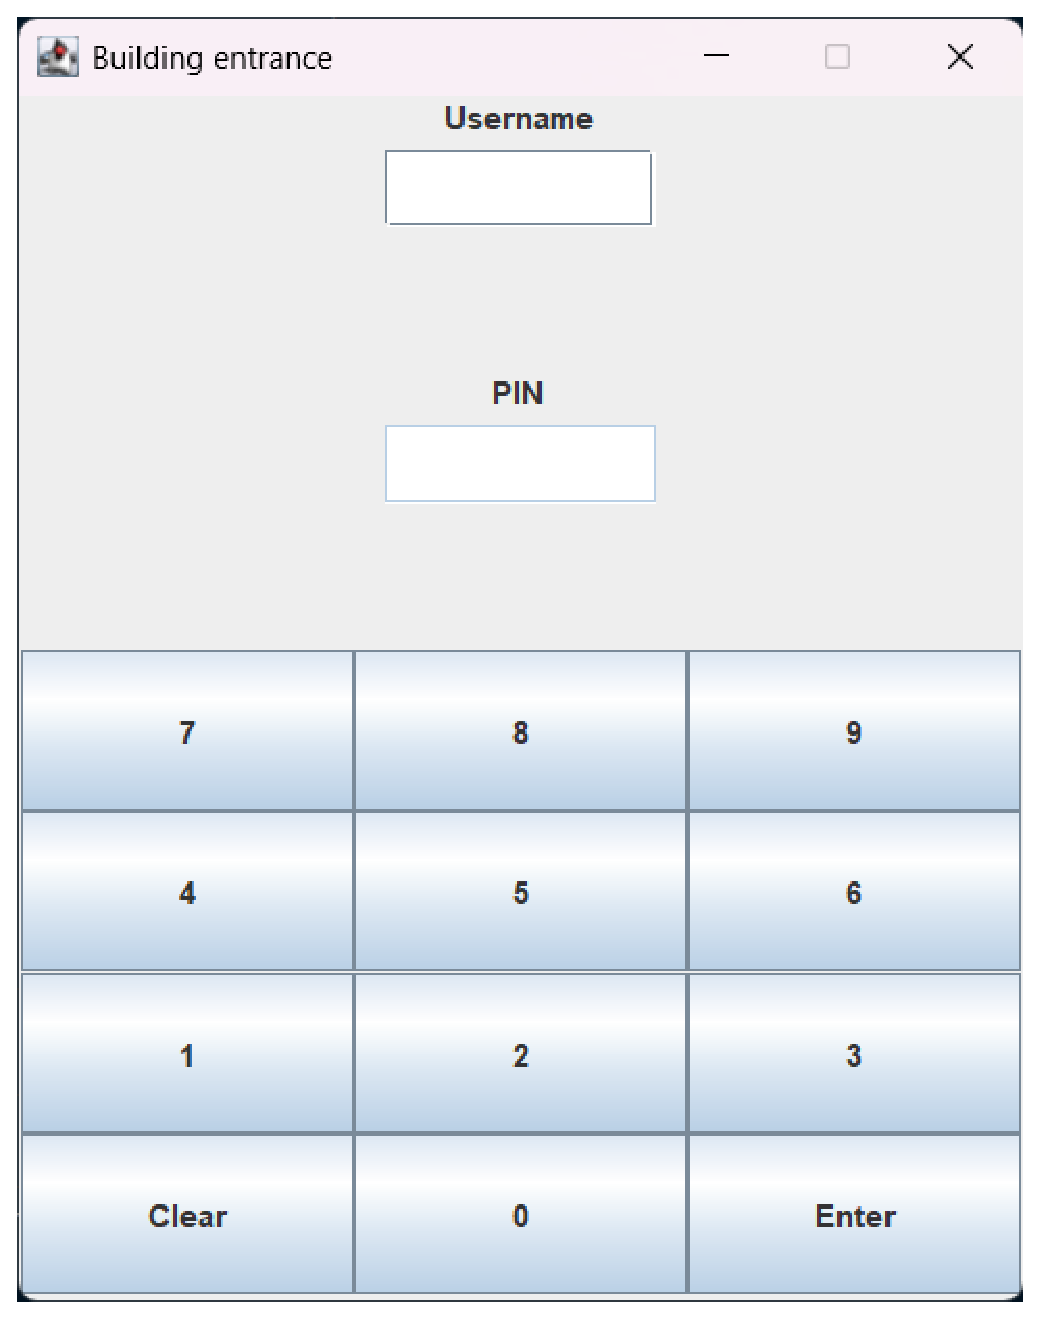
\includegraphics[width=\textwidth,height=0.5\textheight,keepaspectratio]{figures/app-images/panel-logowania.eps}
    \caption{Ekran logowania. \cite{SwingLayouts} \label{fig8}}
\end{figure}

\newpage
\section{Użytkownik (\textit{user})}
\subsection{Panel mieszkańca}
Jest to panel zwykłego użytkownika \textit{user} (Rys. 5.4) do którego użytkownik może się zalogować jeśli jest zarejestrowany w budynku przez 
administratora oraz jeżeli posiada przydzielone mieszkanie. Panel ten wyświetla informacje o mieszkaniu i jego włascicielu oraz pozwala na modyfikowanie parametrów mieszkania, wysyłanie zgłoszeń (Rys 5.5).
Z panelu tego można cofnąć się do panelu logowania poprzez przycisk \textit{Logout}
\begin{figure}[H]
    \centering
    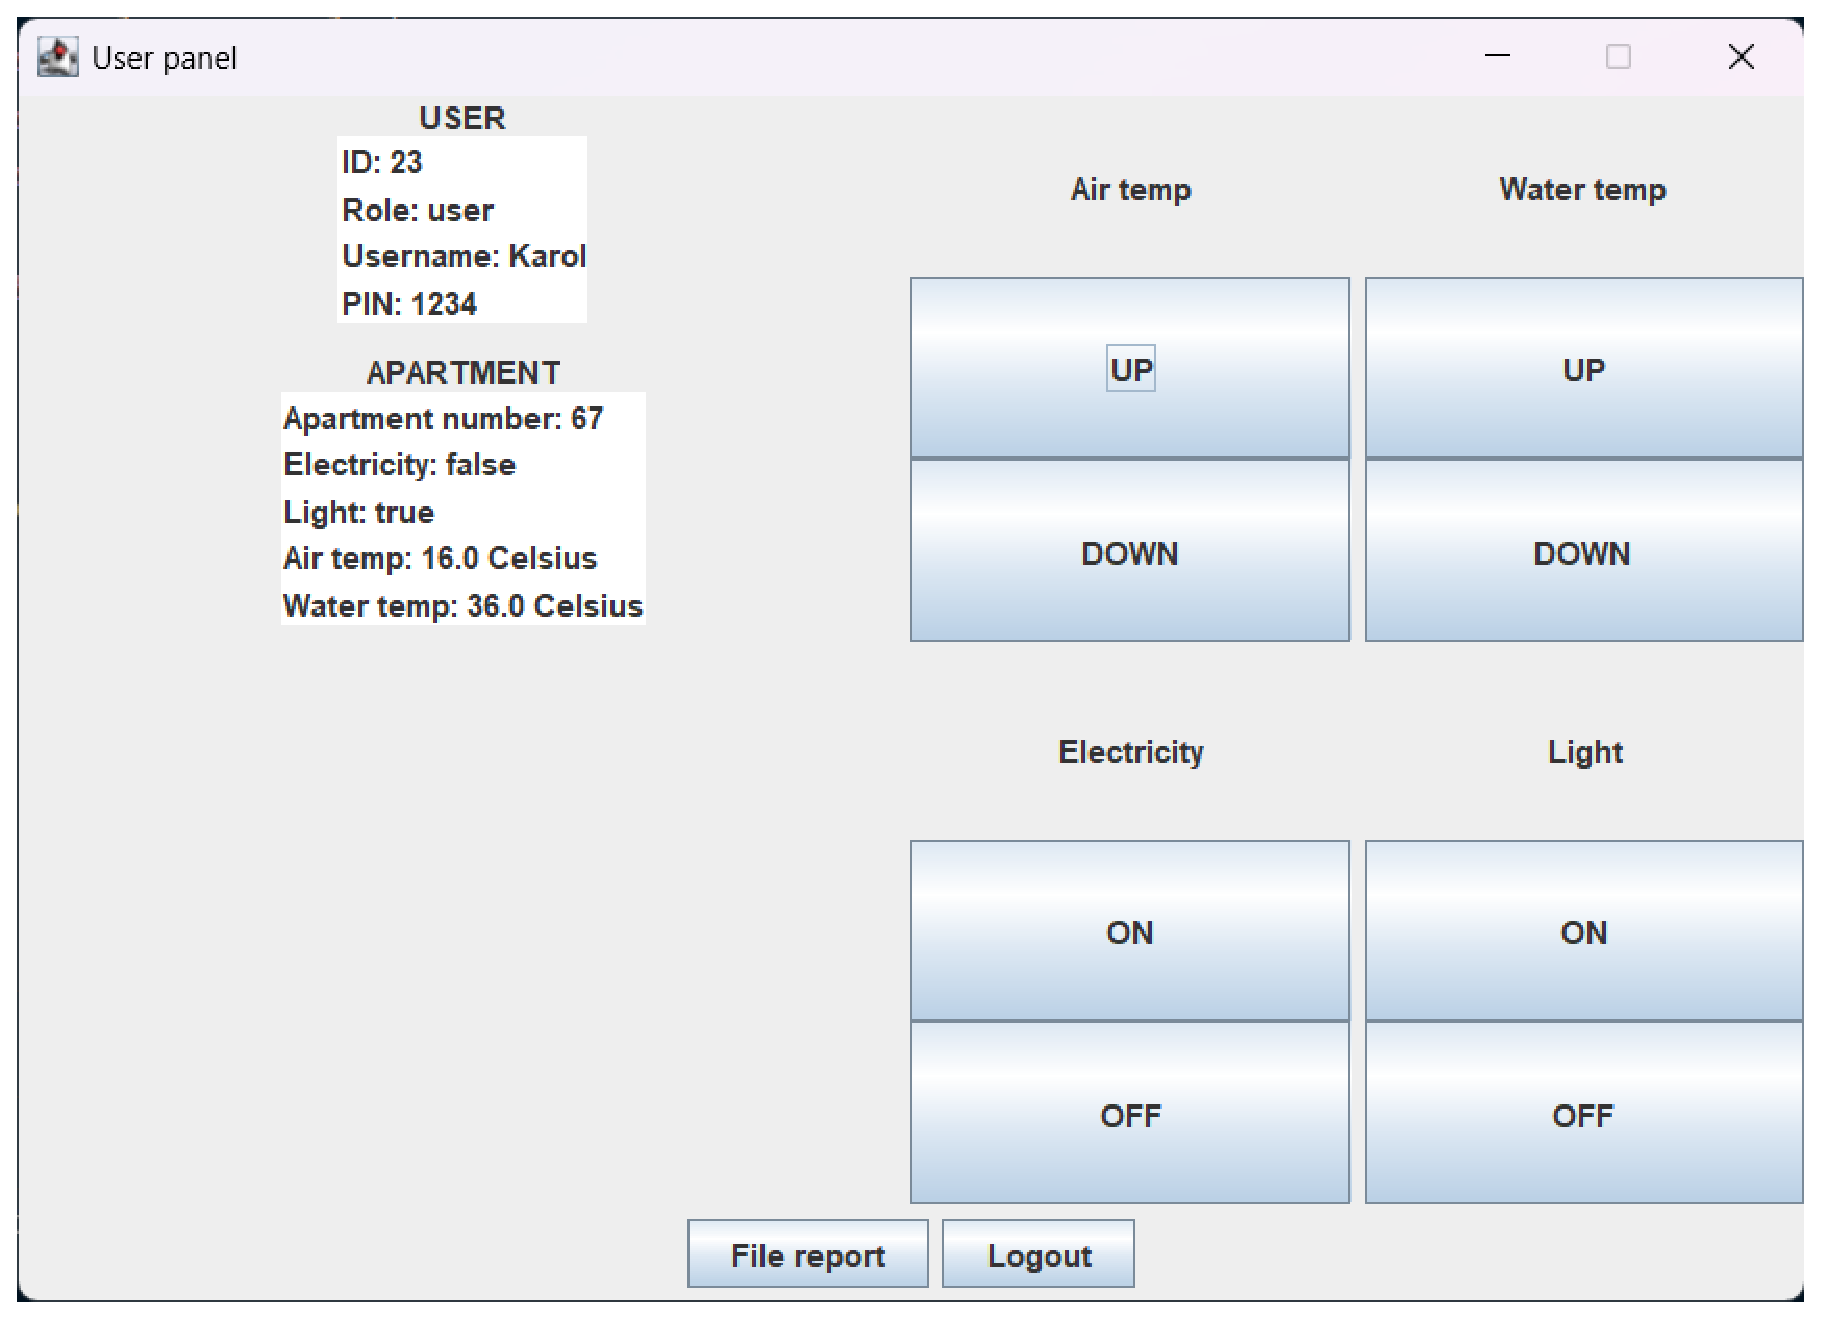
\includegraphics[width=\textwidth,height=0.5\textheight,keepaspectratio]{figures/app-images/user-panel.eps}
    \caption{Panel użytkownika.\label{fig9}}
\end{figure}

\newpage
\subsection{Wysyłania zgłoszeń}
Przycisk \textit{File report} w panelu użytkownika (Rys 5.4) otwiera okno dzięki któremu użytkownik może wysłać zgłoszenie do administratora 
(np. zgłoszenie o problemie w mieszkaniu). Zgłoszenie składa się z ogólnego tematu zgłoszenia oraz jego bardziej szczegółowej treści, następnie 
poprzez przycisk \textit{Send} zgłoszenie zostaje wysłane do administratora. Zamknięcie okna poprzez \textit{X} powoduje powrót do panelu użytkownika.
\begin{figure}[H]
    \centering
    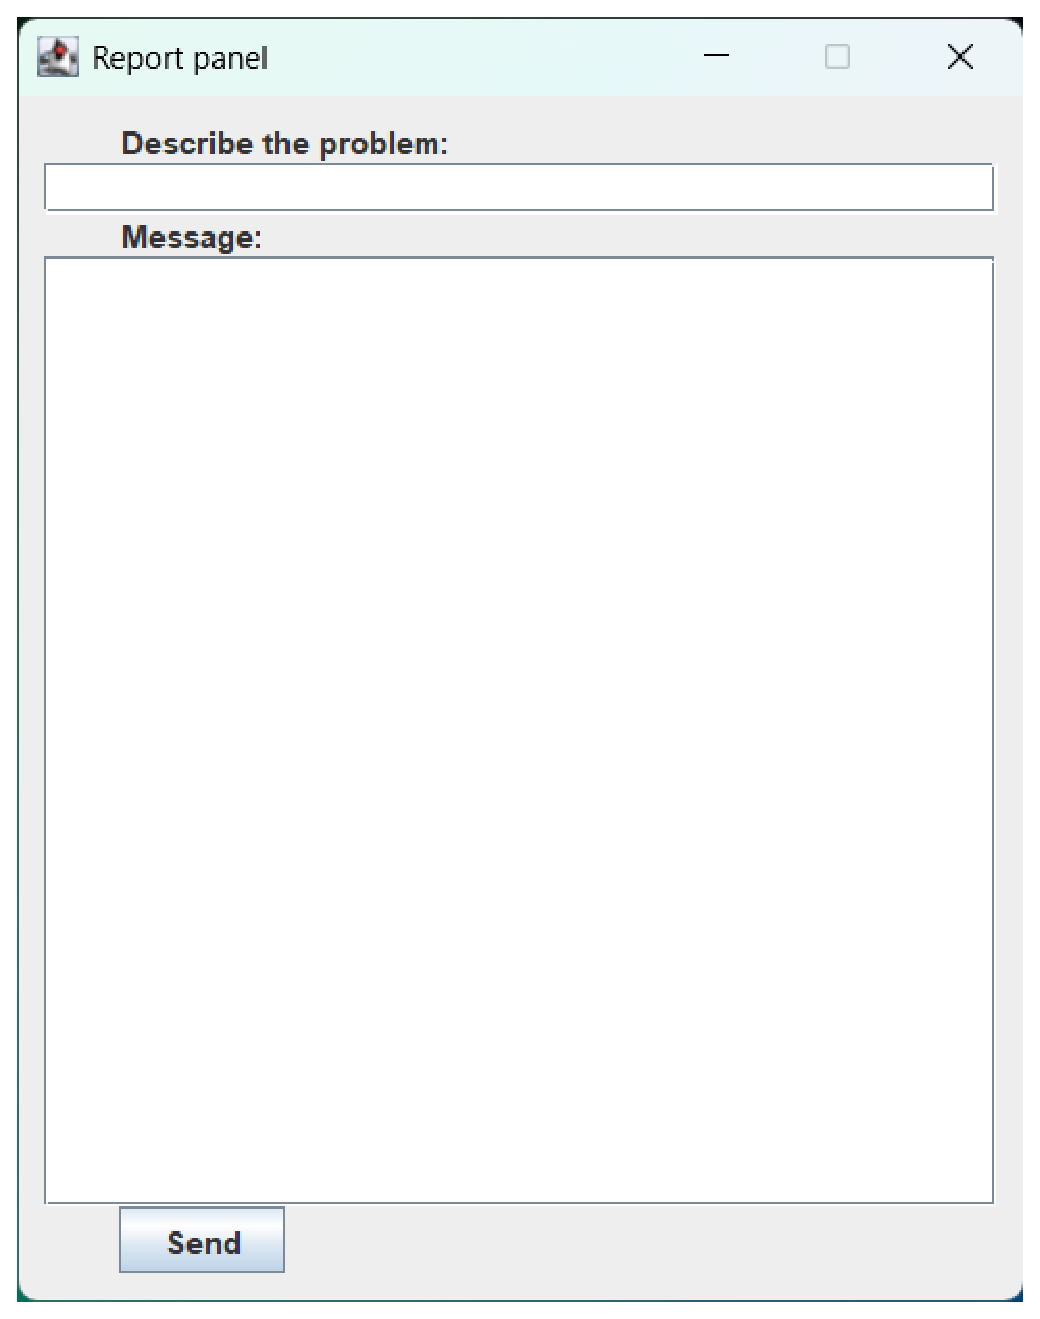
\includegraphics[width=\textwidth,height=0.5\textheight,keepaspectratio]{figures/app-images/user-file-report.eps}
    \caption{Panel wysyłania zgłoszeń.\label{fig10}}
\end{figure}

\newpage
\section{Administrator (\textit{admin})}
\subsection{Panel administratora}
Panel administratora (Rys 5.6) wyświetla użytkowników, mieszkania, zgłoszenia wysłane przez użytkowników.
Przycisk \textit{Logout} powoduje powrót do ekranu logowania a przycisk \textit{CLOSE BUILDING} zamyka budynek nie pozwalając użytkownikom 
wejść do budynku i zmienia się na przycisj \textit{OPEN BUILDING} który otworzy budynek.
\begin{figure}[H]
    \centering
    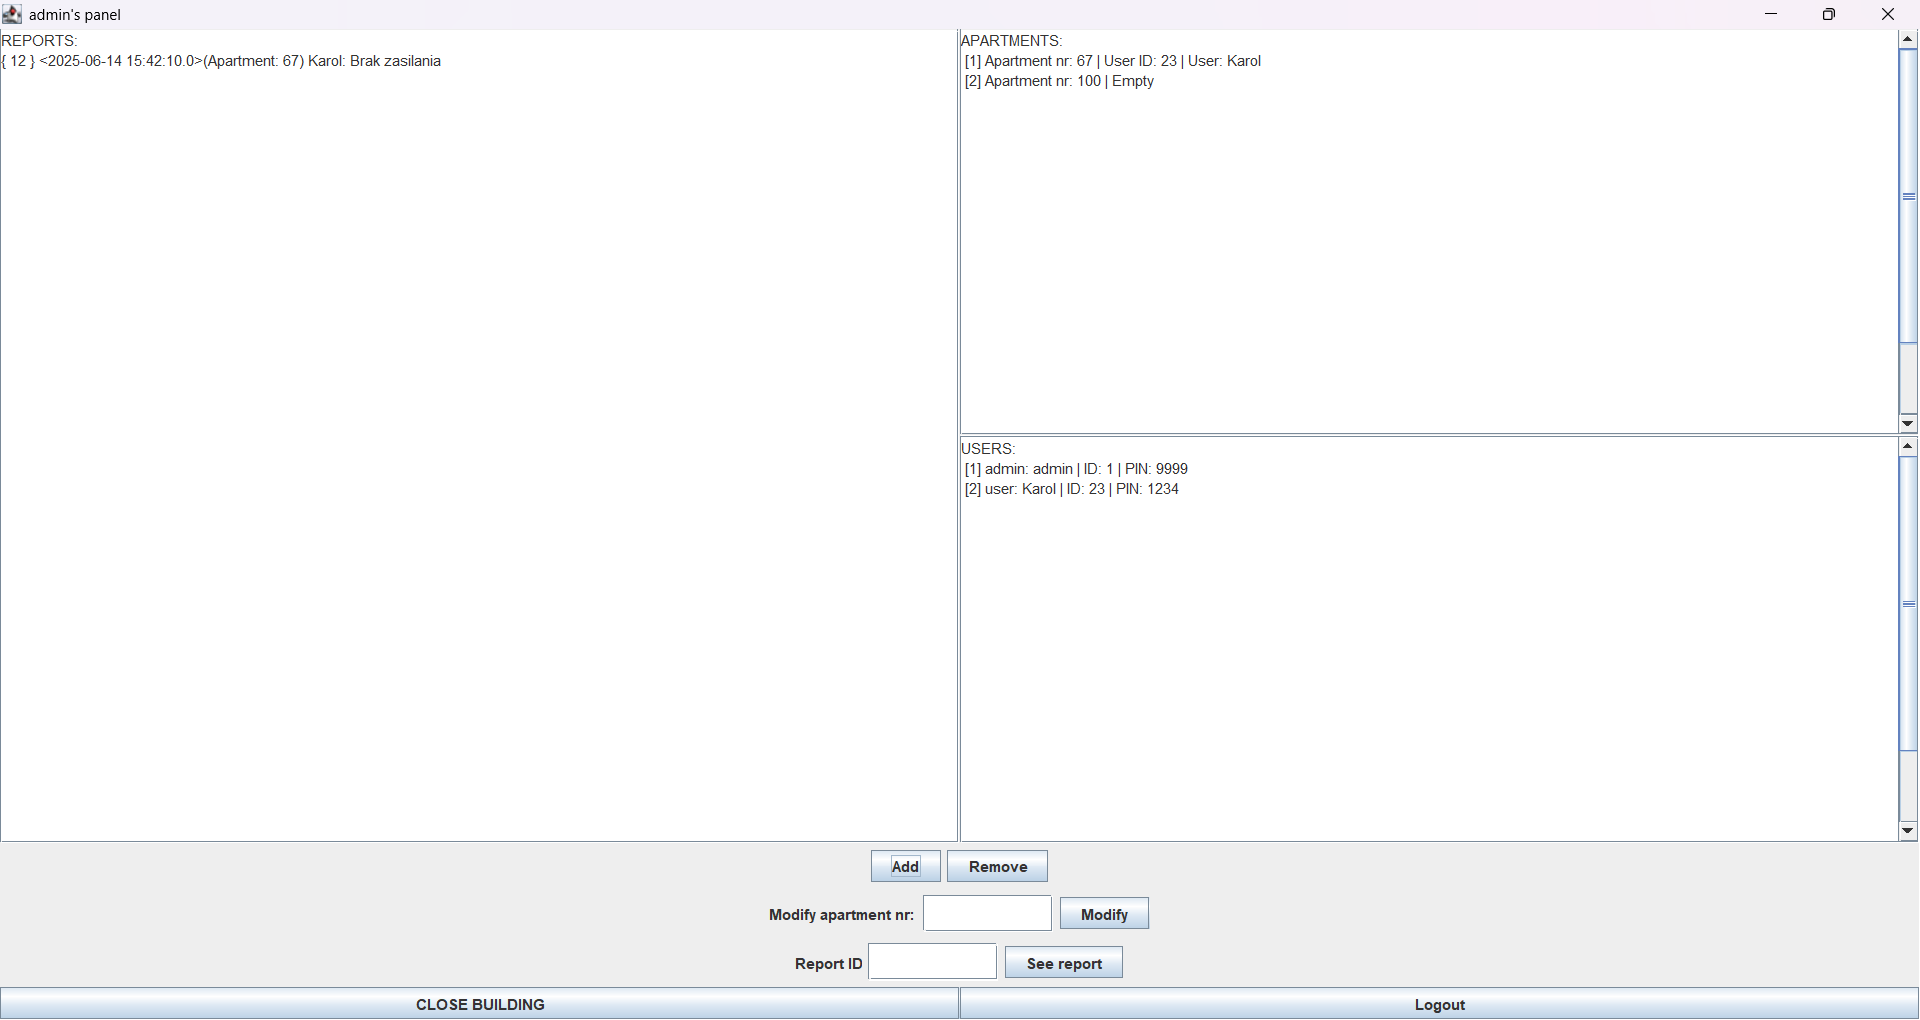
\includegraphics[width=\textwidth,height=0.8\textheight,keepaspectratio]{figures/app-images/admin-panel.eps}
    \caption{Panel administratora.\label{fig11}}
\end{figure}

\newpage
\subsection{Dodawanie obiektów}
Poprzez kliknięcie przycisku \textit{Add} w panelu administratora (Rys 5.6) otworzy się okno dodawania użytkowników, mieszkań 
oraz użytkowników do mieszkań (Rys 5.7, 5.8, 5.9) przełączane przez rozsuwaną listę.

\begin{figure}[H]
    \centering
    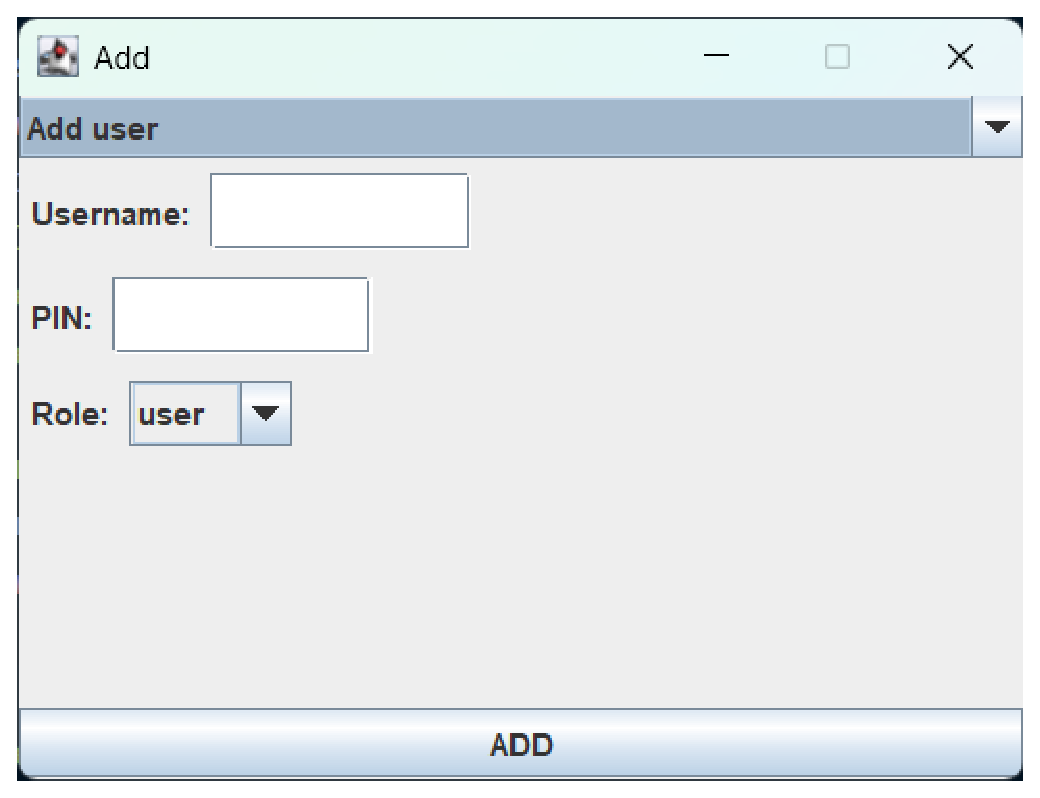
\includegraphics[width=\textwidth,height=0.2\textheight,keepaspectratio]{figures/app-images/Add/add-user.eps}
    \caption{Dodawanie użytkownika.\label{fig12}}
\end{figure}

\begin{figure}[H]
    \centering
    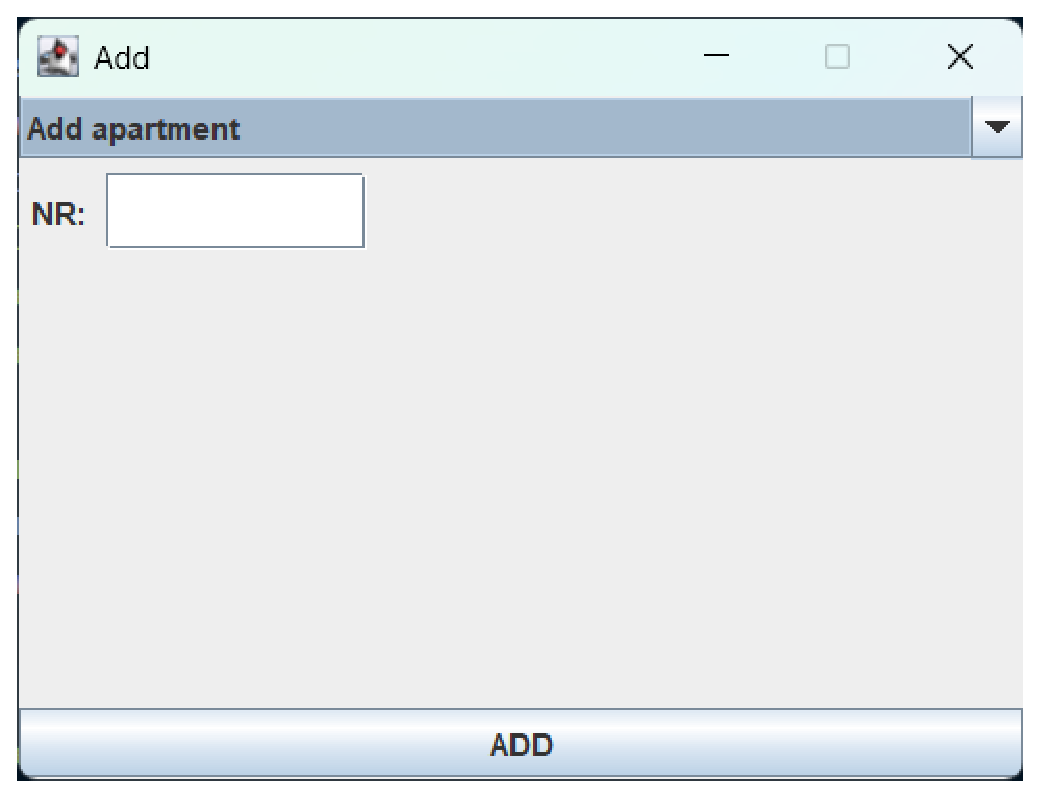
\includegraphics[width=\textwidth,height=0.2\textheight,keepaspectratio]{figures/app-images/Add/add-apartment.eps}
    \caption{Dodawanie mieszkania.\label{fig13}}
\end{figure}

\begin{figure}[H]
    \centering
    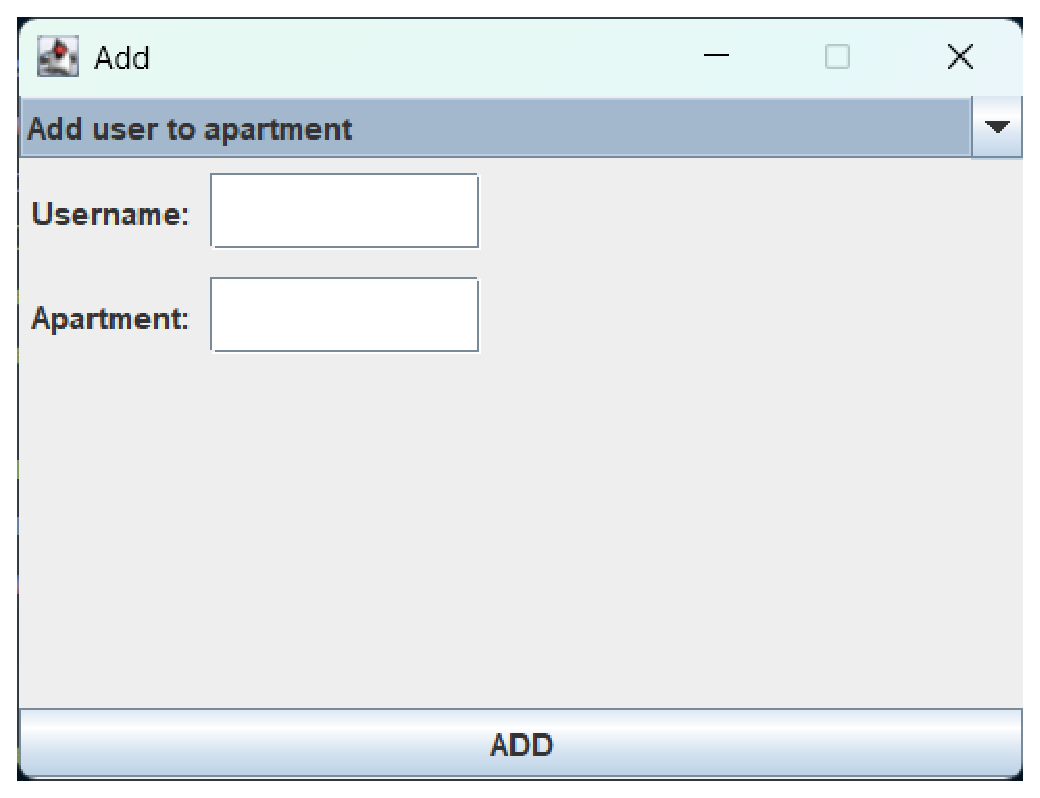
\includegraphics[width=\textwidth,height=0.2\textheight,keepaspectratio]{figures/app-images/Add/add-user-to-apartment.eps}
    \caption{Dodawanie użytkownika do mieszkania.\label{fig14}}
\end{figure}

\newpage
\subsection{Usuwanie obiektów}
Poprzez kliknięcie przycisku \textit{Remove} w panelu administratora (Rys 5.6) otworzy się okno usuwania użytkowników, mieszkań, 
użytkowników z mieszkań oraz zgłoszeń (Rys 5.10, 5.11, 5.12, 5.13) przełączane przez rozsuwaną listę.

\begin{figure}[H]
    \centering
    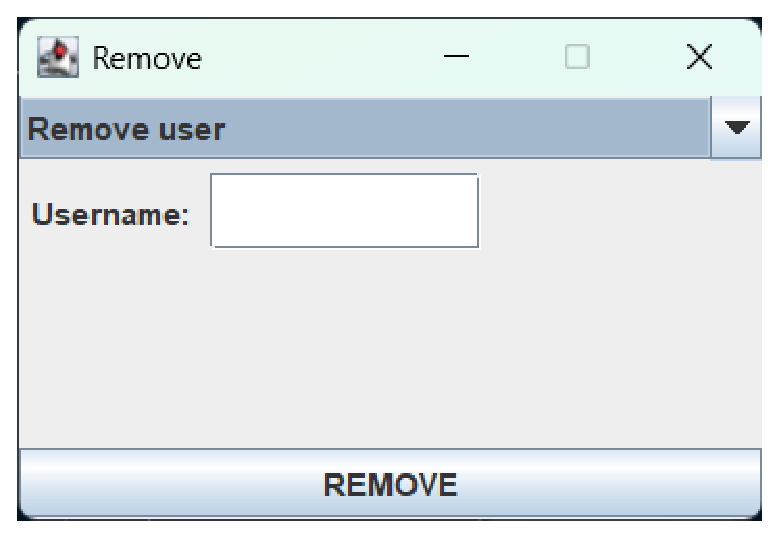
\includegraphics[width=\textwidth,height=0.15\textheight,keepaspectratio]{figures/app-images/Remove/remove-user.eps}
    \caption{Usuwanie użytkownika.\label{fig15}}
\end{figure}

\begin{figure}[H]
    \centering
    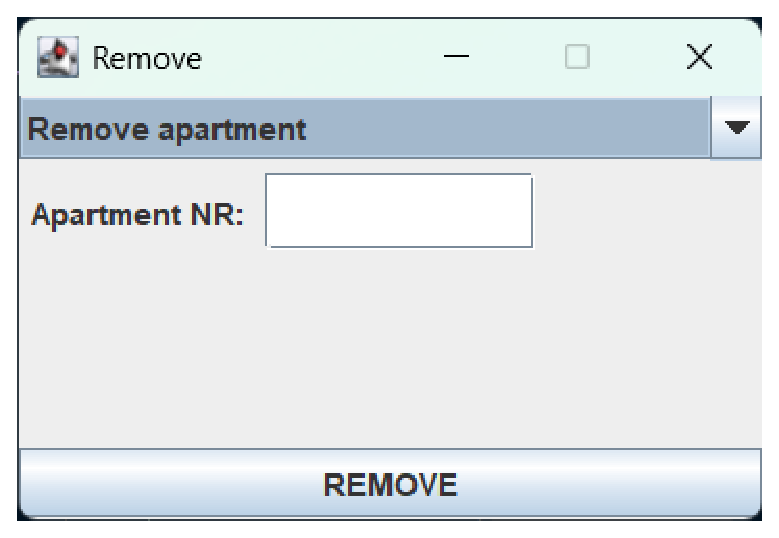
\includegraphics[width=\textwidth,height=0.15\textheight,keepaspectratio]{figures/app-images/Remove/remove-apartment.eps}
    \caption{Usuwanie mieszkania.\label{fig16}}
\end{figure}

\begin{figure}[H]
    \centering
    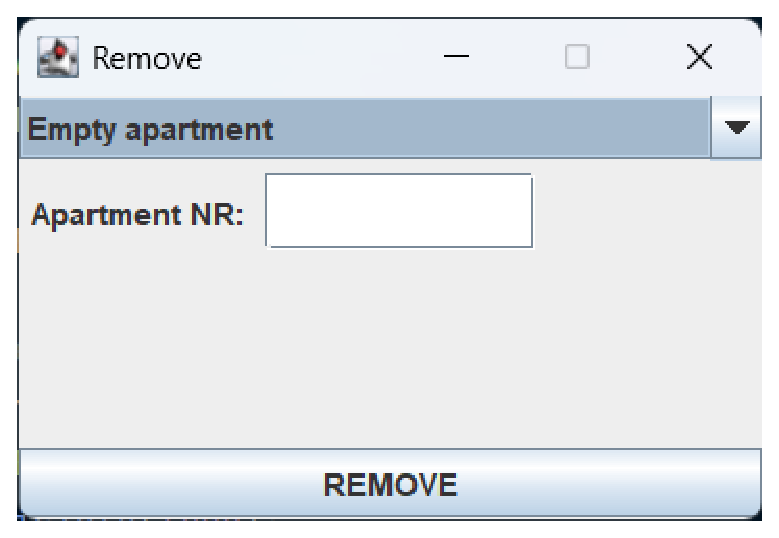
\includegraphics[width=\textwidth,height=0.15\textheight,keepaspectratio]{figures/app-images/Remove/empty-apartment.eps}
    \caption{Usuwanie użytkownika z mieszkania.\label{fig17}}
\end{figure}

\begin{figure}[H]
    \centering
    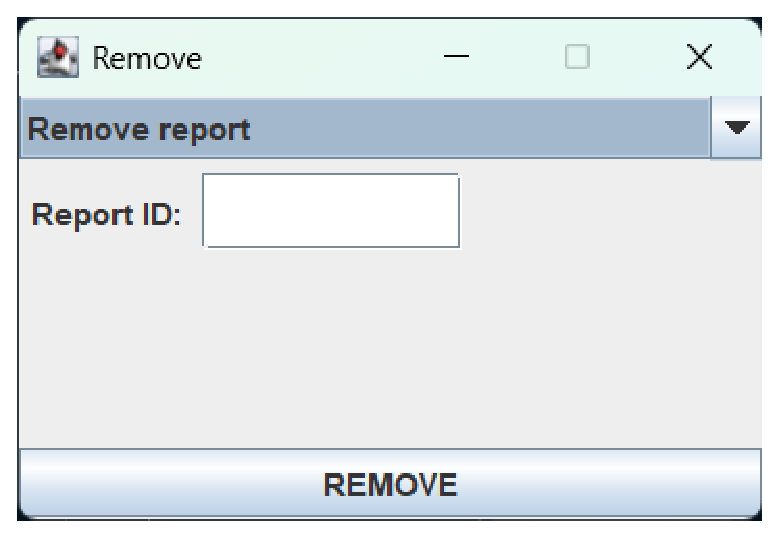
\includegraphics[width=\textwidth,height=0.15\textheight,keepaspectratio]{figures/app-images/Remove/remove-report.eps}
    \caption{Usuwanie zgłoszenia.\label{fig18}}
\end{figure}

\newpage
\subsection{Modyfikowanie parametrów mieszkania}
Poprzez pole \textit{Modify apartment nr:} (Rys 5.14) znajdujące się w panelu administratora (Rys 5.6), poprzez wpisanie numeru mieszkania 
i kliknięciu przycisku \textit{Modify} otworzy się okno które pozwoli na modyfikacje parametrów mieszkania o podanym numerze (Rys 5.15),
np. zmiana temperatury powietrza, wody, włączanie lub wyłączanie światła.

\begin{figure}[H]
    \centering
    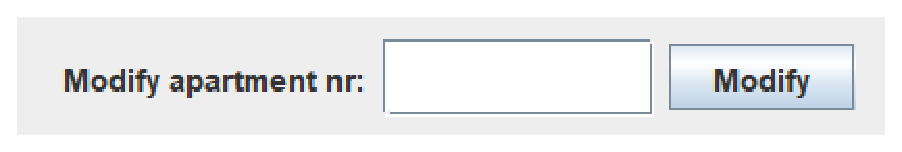
\includegraphics[width=\textwidth,height=0.15\textheight,keepaspectratio]{figures/app-images/admin-panel-modify.eps}
    \caption{Pole \textit{Modify apartment nr:}.\label{fig19}}
\end{figure}

\begin{figure}[H]
    \centering
    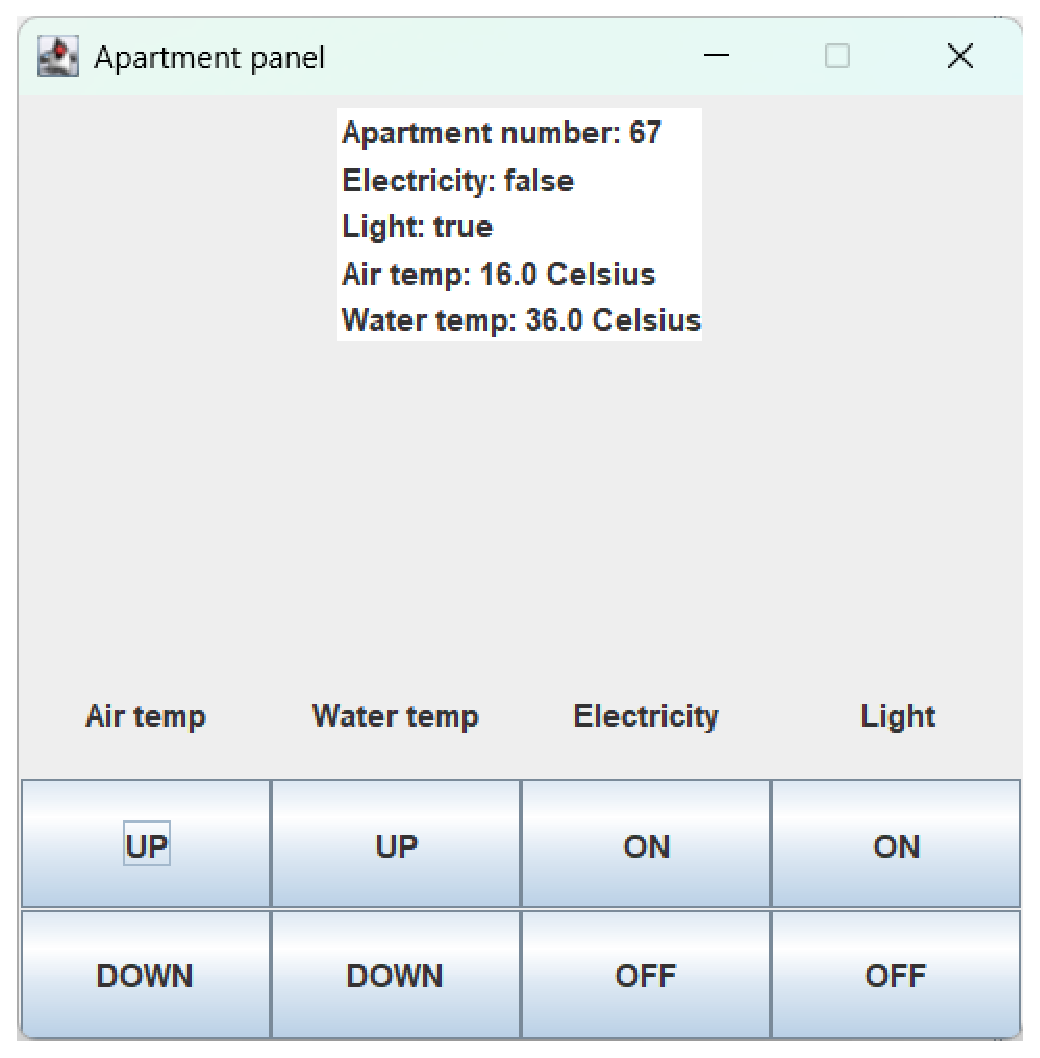
\includegraphics[width=\textwidth,height=0.3\textheight,keepaspectratio]{figures/app-images/modify-apartment.eps}
    \caption{Modyfikacja mieszkania.\label{fig20}}
\end{figure}

\newpage
\subsection{Otwieranie treści zgłoszeń}
Poprzez pole \textit{Report ID} (Rys 5.16) znajdujące się w panelu administratora (Rys 5.6), poprzez wpisanie ID zgłoszenia 
i kliknięciu przycisku \textit{See report} otworzy się okno które wyświetli treść zgłoszenia (Rys 5.17).

\begin{figure}[H]
    \centering
    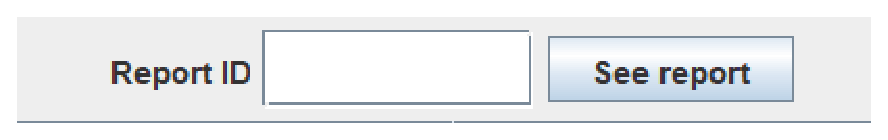
\includegraphics[width=\textwidth,height=0.15\textheight,keepaspectratio]{figures/app-images/admin-panel-report.eps}
    \caption{Pole \textit{Report ID}.\label{fig21}}
\end{figure}

\begin{figure}[H]
    \centering
    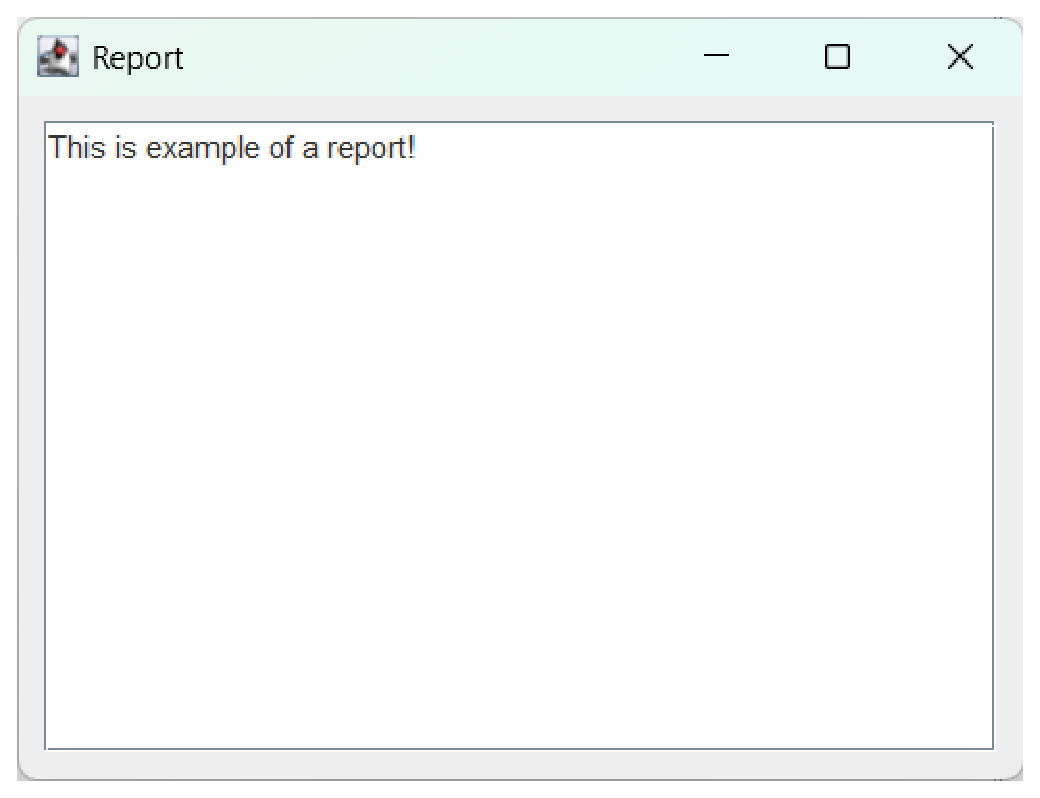
\includegraphics[width=\textwidth,height=0.3\textheight,keepaspectratio]{figures/app-images/see-report.eps}
    \caption{Treść zgłoszenia.\label{fig22}}
\end{figure}
%----------------Podsumowanie
\chapter{Podsumowanie}
\section{Wykonane prace}
\begin{enumerate}
    \item \textbf{Baza danych zawierająca tabele przechowujące dane}
    \item \textbf{Oprawa graficzna pozwalająca na intuicyjne poruszanie się po programie}
    \item \textbf{Funkcje dodawania użytkowników, mieszkań i raportów do bazy danych}
    \item \textbf{Funkcje modyfikujące i pobierające informacje z bazy danych}
\end{enumerate}
\section{Możliwe prace rozwojowe}
\begin{enumerate}
    \item \textbf{Poprawa interfejsu graficznego na bardziej nowoczesny}
    \item \textbf{Poprawa funkcjonalności paneli dodawania i usuwania danych}
    \item \textbf{Rozszerzenie bazy danych o większą liczbę tabel oraz lepsze łączenie między tabelami}
\end{enumerate}
% ********** Koniec **********